\chapter{A Hyper-Lambda-Calculus for Synchronous Communication}
\label{ch:exchange}

\section{Introduction}

We propose a way to unify ML-style programming
languages~\citep{milner1997definition, marlow2010haskell} and
$\pi$-calculus~\citep{milner1999communicating}, which are two of Robin
Milner's achievements.
``Well-typed expressions do not go wrong,'' said \citet{milner1978}.
However, when communication is involved, how to maintain the principle
is not yet settled.
For example, Haskell, which is an ML-style programming language,
allows different threads to communicate using an MVar \texttt{mv} of
type \texttt{MVar
a}, with commands
\texttt{putMVar mv} of type \texttt{a -> IO ()} and \texttt{takeMVar mv}
of type \texttt{IO
a}\footnote{The arrow \texttt{->} shows implication $\imp$ and the tuple
() shows the unit type $\one$}.
The former command consumes an argument of type~\texttt{a} and
the argument appears from the latar command.
However, if programmers make mistakes, these commands can
cause a deadlock in execution time even if the program passes the type
checking.
This is because the type system of Haskell allows programmers to
use only one of $(\phi\imp \one)$ and $\phi$.
Fundamentally, this is because the type system of Haskell
is based on intuitionistic logic, which allows throwing away proofs.

As a remedy, we invent a typed lambda calculus where
the user is forced to use both of sending and receiving primitives each once.
For that we use the technique of linear types:
linear types can specify a portion of program to be used
just once.

We show that it is still possible to build
a type system which is based on a logic.
Wadler and Pfenning did that, but our type system can type processes
which Wadler
and Pfenning's system cannot.

From the standard intuitionistic linear logic,
the only change is adding Amida axiom\index{axiom!Amida}\index{Amida axiom|see{axiom}}
$(\phi\limp\psi)\otimes(\psi\limp\phi)$.
We call the resulting logic Amida logic.
In Amida logic, we can express $\pi$-calculus-like processes as macros.
To be honest, our initial motivation was just studying the axiom
$(\phi\limp\psi)\otimes(\psi\limp\phi)$%
\footnote{Takeuti Izumi asked about conjunctions
after the author talked about $(\phi\limp\psi)\oplus (\psi\limp\phi)$.}.
A natural way to add $(\phi\limp\psi)\otimes(\psi\limp\phi)$ as an axiom
is adding a pair of primitives $c,\co c$ so that
$\cdots ct \cdots \co c u \cdots$ reduces to
$\cdots u  \cdots t \cdots$: in words,
$c$ outputs $\co c$'s input and vice versa.
We can obtain the send-receive communication when we specialize the
axiom as $(\phi\limp \one)\otimes(\one\limp\phi)$.  The left hand side
$\tj{c}{\phi\limp\one}$ is the sending primitive and
the right hand side $\tj{\co c}{\one \limp\phi}$ is the receiving
primitive.

When we want to use these primitives anywhere in lambda terms,
there is one problem: what happens to $\co c(c t)$?
In this case, we do not know the output of $c$ because we only have an
equality between $\co c$'s input and $c$'s output.
Fortunately, we just want to know the output of $\co c$, which is the
input of $c$, that is, $t$.
In a more complicated case $\co c(\co d(c (d t)))$,
we can reason the output of $\co c$ as the input of $c$ as the output of
$d$ as the input of $\co d$ as the output of $c$ as the input of $\co c$
as the output of $\co d$ as the input of $d$, which is $t$.

We have more questions.
\begin{itemize}
 \item Due to addition of the axiom, is it the case that
       every type is inhabited?  In other words,
      is the resulting type system consistent (Sect.~\ref{sec:convergence})?
 \item How does it generalize over channels having more complicated
       protocols (Sect.~\ref{sec:session-process})?
 \item Can we implement process calculi using the aforementioned
       primitives (Sect.~\ref{sec:session-process})?
\end{itemize}

After following these practical questions,
we proceed to developing a proof net structure for the logic.
It turns out that the the ``Amida lottery,'' which is a traditional
Japanese way of making arbitrary permutations, provides the answer.

Japanese schoolchildren use \textit{Amida lotteries}\index{Amida lotteries}
for assigning seats, jobs, teams and so on to classmates.

\fix{add}

The diagram defines a permutation.
From a top end, one can find the counterpart by following the vertical
line, but one has to cross the bridge whenever one finds one and then
after crossing the bridge, one has to go down the vertical line.


\section{Definitions}

\subsection{Types}
For a set $S$, we define $\phi\in\form(S)$ by BNF:
\[
 \phi::=s\mid \one \mid X \mid \phi\otimes\phi\mid \phi\limp\phi\mid
 \phi\oplus\phi\mid \phi\with\phi\mid \bang\phi\mid \forall X.\phi
\]
where $s$ is an element of $S$ and $X$ is a propositional variable.
The propositional variable in the last clause is binding.
A \textit{type}\index{type} is an element of $\form(\emptyset)$.
A \textit{formula}\index{formula} is a type.

\subsection{Terms and Free Variables}

Following Abramsky's linear lambda calculus
LF~\citep{abramsky1993computational}, we first define patterns
binding sets of variables:
\begin{itemize}
 \item $\ast$ and $\_$ are patterns binding $\emptyset$,
 \item $\lpair{x,\_}$, $\lpair{\_,x}$ and $\bang x$ are patterns binding
       $\{x\}$,
 \item $x\otimes y$ and $x@y$ are patterns binding $\{x,y\}$.
\end{itemize}
We write $BV(p)$ for the set of bound variables of pattern~$p$.
Using patterns, we define a term $t$ with free variables~$S$.
We assume countably infinitely many \textit{channels}\index{channel}
with involution
satisfying $\co c\neq c$ and $\co{\co c} = c$.
\begin{itemize}
 \item a variable $x$ is a term with free variables $\{x\}$,
 \item if $t$ is a term with free variables~$S$, $u$ is a term with
       free variables~$S'$ and $S$ and $S'$ are disjoint, $t\otimes u$ and
       $tu$ are terms with free variables $S\cup S'$,
 \item if $t$ and $u$ are terms with free variables $S$, then
       $\lpair{t,u}$ is a term with free variables~$S$,
 \item if $t$ is a term with free variables~$S$, then
       $\inl x, \inr t$ and $\bang t$ are terms with free variables~$S$
 \item if $t$ is a term with free variables $S\cup \{x\}$ and $x$ is not
       in $S$, then $\lambda x.t$ is a term with free variables~$S$,
 \item if $t$ is a term with free variables~$S$, $p$ is a pattern
       binding $S'$, $u$ is a term with free variables $S'\cup S''$ and
       $S\cap S'' = S'\cap S'' = \emptyset$, then,
       $\letin t p u$ is a term with free variables $S\cup S''$,
 \item if $t$ is a term with free variables $S$,
       $u$ is a term with free variables $S''\cup \{x\}$,
       $v$ is a term with free variables $S''\cup \{y\}$,
       $x,y\notin S''$ and $S\cap S'' = \emptyset$,
       $\mat t x u y v$ is a term with free variables $S\cup S''$, and
 \item channels are terms with free variables~$\emptyset$.
\end{itemize}
Note that a term with free variables $S$ is not a term with free
variables $S'$ when $S\neq S'$.  Only the last clause is original,
introducing channels, which are our communication primitives.
We introduce an abbreviation
\begin{align*}
 \ign \epsilon t   & \equiv t\\
 \ign {s_0,\vec s} t & \equiv \letin {s_0} \ast {\ign {\vec s} t}
\end{align*}
inductively for a sequence of terms~$\vec s$.
$\epsilon$ stands for the empty sequence.
The symbol $\mathsf{ign}$ is intended to be pronounced ``ignore''.

\subsection{Typing Derivations}

On top of Abramsky's linear lambda calculus
LF~\citep{abramsky1993computational}\index{LF}, we add a rule to
make $(\phi\limp\psi)\otimes(\psi\limp\phi)$ inhabited. \fix{define
inhabited somewhere}
A \textit{context}\index{context}~$\G$ is a possibly empty sequence of
variables associated with
types where the same variable appears at most once.
A context $\tj{x}{X}, \tj{y}{Y}$ is allowed, but $\tj{x}{X}, \tj{x}{Y}$
and $\tj{x}{X},\tj{x}{X}$ are not contexts.
A \textit{hypersequent}\index{hypersequent} is inductively defined as
\begin{align*}
 \hypert ::=\, &\G\tr\tj{t}{\phi}
 \mid\, (\hypert\hmid \hypert)
\end{align*}
where $\G$ is a context.
In this chapter, we interpret the components conjunctively.
We name this technique the \textit{conjunctive
hypersequent}\index{hypersequent!conjunctive}.

Differently from the previous
papers~\citep{avron91,Baaz01122003,avrontableau,avron96},
here, the hypersequent $\G\tr\phi\hmid \D\tr\psi$ is interpreted as the
conjunction of components:
$(\bigotimes\G\limp\phi)\otimes (\bigotimes\D\limp\psi)$.

The typing rules are in Figure~\ref{fig:exchange:rules}.
 \begin{figure}
  \centering
  % axiom
  \AxiomC{}
  \LL{Ax}
  \UnaryInfC{$\tj{x}{\phi}\tr\tj{x}{\phi}$}
  \DisplayProof
  %
  \hfill
  \AxiomC{$\hypert$}
  \AxiomC{$\hypert'$}
  \LL{merge}
  \BinaryInfC{$\hypert\hmid\hypert'$}
  \DisplayProof
  % cut XXX is this necessary?; yes
  \hfill
  \AxiomC{$\hypert\hmid\G\tr\tj{t}{\phi}\hmid\tj{x}{\phi},\D\tr\tj{u}{\psi}$}
  \LL{Cut}
  \UnaryInfC{$\hypert\hmid\G,\D\tr\tj{u[t/x]}{\psi}$}
  \DisplayProof
  \ruleskip
  % exchange
  \AxiomC{$\hypert\hmid\G,\tj{x}{\phi},\tj{y}{\psi},\D\tr\tj{t}{\theta}$}
  \LL{IE}
  \UnaryInfC{$\hypert\hmid\G,\tj{y}{\psi},\tj{x}{\phi},\D\tr\tj{t}{\theta}$}
  \DisplayProof
  %
  \hfill
  \AxiomC{$\hypert\hmid \G \tr\tj t\phi \hmid \D \tr\tj u\psi\hmid \hypert'$}
  \LL{EE}
  \UnaryInfC{$\hypert\hmid \D \tr\tj u\psi \hmid \G \tr\tj t\phi \hmid \hypert'$}
  \DisplayProof
  \ruleskip
  %
  \ruleskip
  % 1R
  \AxiomC{}
  \LL{$\one$R}
  \UnaryInfC{$\tr\tj{\ast}{\one}$}
  \DisplayProof
  %
  \hfill
  % 1L
  \AxiomC{$\hypert\hmid\G\tr\tj{t}{\phi}$}
  \LL{$\one$L}
  \UnaryInfC{$\hypert\hmid\G,\tj{z}{\one}\tr\tj{\ign z t}{\phi}$}
  \DisplayProof
  %
  \hfill
  % otimes R
  \AxiomC{$\hypert\hmid\G\tr\tj{t}{\phi}\hmid\D\tr\tj{u}{\psi}$}
  \LL{$\otimes$R}
  \UnaryInfC{$\hypert\hmid\G,\D\tr\tj{t\otimes u}{\phi\otimes \psi}$}
  \DisplayProof
  %
  \ruleskip
  % Sync
  \AxiomC{$\hypert\hmid\G\tr\tj{t}{\phi}\hmid \D\tr\tj{u}{\psi}$}
  \LL{Sync}
  \UnaryInfC{$\hypert\hmid
  \G\tr\tj{ct}{\psi}\hmid \D\tr\tj{\co cu}{\phi}$}
  \DisplayProof
  %
  \hfill
  % otimes L
  \AxiomC{$\hypert\hmid\G,\tj{x}{\phi},\tj{y}{\psi}\tr\tj{t}{\theta}$}
  \LL{$\otimes$L}
  \UnaryInfC{$\hypert\hmid\G,\tj{z}{\phi\otimes\psi}\tr\tj{\letin{z}{x\otimes
  y}{t}}{\theta}$}
  \DisplayProof
  %
  \ruleskip
  % limp R
  \AxiomC{$\hypert\hmid\G,\tj{x}{\phi}\tr\tj{t}{\psi}$}
  \LL{$\limp$R}
  \UnaryInfC{$\hypert\hmid\G\tr\tj{\lambda x.t}{\phi\limp \psi}$}
  \DisplayProof
  %
  \hfill
  % limp L
  \AxiomC{$\hypert\hmid\G\tr\tj{t}{\phi}\hmid\tj{x}{\psi},\D\tr\tj{u}{\theta}$}
  \LL{$\limp$L}
  \UnaryInfC{$\hypert\hmid\G,\tj{f}{\phi\limp\psi},\D\tr \tj{u[(ft)/x]}{\theta}$}
  \DisplayProof
  %
  \ruleskip
  % andR
  \AxiomC{$\G\tr\tj{t}{\phi}$}
  \AxiomC{$\G\tr\tj{u}{\psi}$}
  \LL{$\with$R}
  \BinaryInfC{$\G\tr\tj{\lpair{t,u}}{\phi\with\psi}$}
  \DisplayProof \\
  %
  \ruleskip
  % andL0
  \AxiomC{$\hypert\hmid\G,\tj{x}{\phi}\tr\tj{t}{\theta}$}
  \LL{$\with$L$_0$}
  \UnaryInfC{$\hypert\hmid\G,\tj{z}{\phi\with\psi}\tr\tj{\letin{z}{\lpair{x,\_}}{t}}{\theta}$}
  \DisplayProof
  %
  \ruleskip
  % andL1
  \AxiomC{$\hypert\hmid\G,\tj{y}{\psi}\tr\tj{t}{\theta}$}
  \LL{$\with$L$_1$}
  \UnaryInfC{$\hypert\hmid\G,\tj{z}{\phi\with\psi}\tr\tj{\letin{z}{\lpair{\_,y}}{t}}{\theta}$}
  \DisplayProof
  %
  \ruleskip
  % oplus R0
  \AxiomC{$\hypert\hmid\G\tr\tj{t}{\phi}$}
  \LL{$\oplus$R$_0$}
  \UnaryInfC{$\hypert\hmid\G\tr\tj{\inl{t}}{\phi\oplus\psi}$}
  \DisplayProof
  %
  \hfill
  % oplus R1
  \AxiomC{$\hypert\hmid\G\tr\tj{u}{\psi}$}
  \LL{$\oplus$R$_1$}
  \UnaryInfC{$\hypert\hmid\G\tr\tj{\inr{u}}{\phi\oplus\psi}$}
  \DisplayProof
  %
  \ruleskip
  % oplus L
  \AxiomC{$\hypert \hmid \G,\tj{x}{\phi}\tr\tj{u}{\theta}\hmid
  \G,\tj{y}{\psi}\tr\tj{v}{\theta}$}
  \LL{$\oplus$L}
  \UnaryInfC{$\hypert\hmid\G,\tj{z}{\phi\oplus\psi}\tr\tj{\mat{z}{x}{u}{y}{v}}{\theta}$}
  \DisplayProof
  %
  \ruleskip
  % !R
  \AxiomC{$\bang\hypert\hmid\bang\G\tr\tj{t}{\phi}$}
  \LL{$\bang$R}
  \UnaryInfC{$\bang\hypert\hmid\bang\G\tr\tj{\bang t}{\bang \phi}$}
  \DisplayProof
  where $\bang\hypert$ contains only components typed $\bang\D\tr \bang\psi$.
  %
  \ruleskip
  % dereliction
  \AxiomC{$\hypert\hmid\G,\tj{x}{\phi}\tr\tj{t}{\psi}$}
  \LL{Dereliction}
  \UnaryInfC{$\hypert\hmid\G,\tj{z}{\bang\phi}\tr\tj{\letin{z}{\bang x}{t}}{\psi}$}
  \DisplayProof
  %
  \ruleskip
  % contraction
  \AxiomC{$\hypert\hmid\G,\tj{x}{\bang\phi},\tj{y}{\bang\phi}\tr\tj{t}{\psi}$}
  \LL{Contraction}
  \UnaryInfC{$\hypert\hmid\G,\tj{z}{\bang\phi}\tr\tj{\letin{z}{x@y}{t}}{\psi}$}
  \DisplayProof
  %
  \ruleskip
  % weakening
  \AxiomC{$\hypert\hmid\G\tr\tj{t}{\psi}$}
  \LL{Weakening}
  \UnaryInfC{$\hypert\hmid\G,\tj{z}{\bang\phi}\tr\tj{\letin{z}{\_}{t}}{\psi}$}
  \DisplayProof
  %
  \ruleskip
  % forall R
  \AxiomC{$\hypert\hmid\G\tr\tj{t}{\phi}$}
  \LL{$\forall$R}
  \UnaryInfC{$\hypert\hmid\G\tr\tj{t}{\forall X.\phi}$}
  \DisplayProof (No free $X$ appears in $\G$ or $\hypert$)
  %
  \hfill
  % forall L
  \AxiomC{$\hypert\hmid\G,\tj{x}{\phi[\psi/X]}\tr\tj{t}{\phi}$}
  \LL{$\forall$L}
  \UnaryInfC{$\hypert\hmid\G,\tj{x}{\forall X.\phi}\tr\tj{t}{\phi}$}
  \DisplayProof
  %
  \ruleskip
  %
  \caption{Most rules are taken from Abramsky~\citep{abramsky1993computational}.
  The Sync rule is original.   $\with$R only
  applicable to singleton hypersequents.}
  \label{fig:exchange:rules}
 \end{figure}
For example,
the formula $(\phi\limp\psi)\otimes(\psi\limp\phi)$ is realized by
the following derivation.
 \begin{center}
  \AxiomC{}
  \UnaryInfC{$\tj{x}{\phi}\tr\tj{x}{\phi}$}
  \AxiomC{}
  \UnaryInfC{$\tj{y}{\psi}\tr\tj{y}{\psi}$}
  \BinaryInfC{$\tj{x}{\phi}\tr\tj{x}{\phi} \hmid
  \tj{y}{\psi}\tr\tj{y}{\psi}$}
  \UnaryInfC{$ \tj{x}{\phi}\tr\tj{cx}{\psi} \hmid \tj{y}{\psi}
  \tr\tj{\co c y}{\phi}$}
  \UnaryInfC{$ \tr\tj{\lambda x.cx}{\phi\limp\psi} \hmid \tj{y}{\psi}
  \tr\tj{\co c y}{\phi}$}
  \UnaryInfC{$ \tr\tj{\lambda x.cx}{\phi\limp\psi} \hmid
  \tr\tj{\lambda y.\co c y}{\phi\limp\phi}$}
  \UnaryInfC{$ \tr\tj{{(\lambda x.cx) \otimes (\lambda y.\co c
  y)}}{(\phi\limp\psi)\otimes(\phi\limp\phi)}$}
  \DisplayProof
 \end{center}
Another example shows how we can type the term $\co c(c x)$.
 \begin{center}
\AxiomC{$\tj{x}{\phi}\tr\tj{x}{\phi}$}
\AxiomC{$\tj{y}{\psi}\tr\tj{y}{\psi}$}
\BinaryInfC{$\tj{x}{\phi}\tr\tj{x}{\phi} \hmid
\tj{y}{\psi}\tr\tj{y}{\psi} $}
\UnaryInfC{
$\tj{x}{\phi}\tr\tj{cx}{\psi} \hmid
\tj{y}{\psi}\tr\tj{\co cy}{\phi} $
}
\LL{(Cut)}
\UnaryInfC{
$\tj{x}{\phi}\tr\tj{\co c(cx)}{\phi}$
}
\DisplayProof
 \end{center}

\subsection{Evaluation Relation}

The set of canonical forms remains the same as Abramsky's
LF~\citep{abramsky1993computational}:
\[
 \lpair{t,u}\qquad \bang t\qquad \ast\qquad v\otimes w\qquad \lambda
 x.t\qquad \inl{v}\qquad\inr{w}
\]
where $v$ and $w$ are canonical forms.

An evaluation hypersequent $\hypere$ is defined by the following
grammar:
\[
 \hypere ::= t\eval_S t\mid (\hypere\hmid \hypere)
\]
where $S$ is a finite set of variables.

Now we define evaluation as a set of evaluation hypersequents
(Figure~\ref{fig:eval}).
Most rules are similar to those of Abramsky's
LF~\citep{abramsky1993computational}.
We add the semantics for channels.

For the sake of \thref{eval-subst} (which will be used for
\thref{thm:generalconvergence} and then consistency), we have to
evaluate a closed subterm~$s$ in
$\lambda
x.t[s/y]$ while Abramsky never evaluated
anything inside lambda.
We decided to evaluate every closed subterms even they are in the
body~$M$ of a lambda abstraction $\lambda x.M$
because channels can appear in the body of lambda-abstraction.
In order to keep track of that, we annotate the $\eval$ relation with
involved free variables~$S$.

 \begin{proposition}
  If evaluation hypersequent $\hypere\hmid t\eval_S v$
  is derivable, $S$ is identical to the set of free variables of $t$.
 \end{proposition}
 \begin{proof}
  Inductively on the evaluation derivations.
 \end{proof}

 The components in the hypersequent represent concurrently running
 processes.
 Thus, the evaluation derivation can be reordered in the following
 manner.
 We call this move moving $R$ upwards.
  \begin{proposition}
   \fix{state}
  \end{proposition}
  \begin{proof}
   \fix{prove}
  \end{proof}

 \begin{figure}
  \centering
  % ast
  \AxiomC{}
  \UnaryInfC{$\ast\eval_\emptyset \ast$}
  \DisplayProof
  \hfill
  \AxiomC{}
  \UnaryInfC{$x\eval_{\{x\}} x$}
  \DisplayProof
  \hfill
  % ast elim
  \AxiomC{$\hypere\hmid t\eval_\emptyset \ast \hmid u\eval_S v$}
  \UnaryInfC{$\hypere\hmid \ign t u\eval_S v$}
  \DisplayProof
  \hfill
  % otimes
  \AxiomC{$\hypere\hmid t\eval_S v\hmid u\eval_{S'} w$}
  \UnaryInfC{$\hypere\hmid t\otimes u\eval_{S\sqcup S'} v\otimes w$}
  \DisplayProof
  \ruleskip
  % ign_not yet
  \AxiomC{$\hypere\hmid t\eval_S t'\hmid u\eval_{S'} u'$}
  \UnaryInfC{$\hypere\hmid \ign t u \eval_{S\sqcup S'} \ign{t'}{u'}$}
  \DisplayProof
  \hfill
  % otimes elim
  \AxiomC{$\hypere\hmid t\eval_\emptyset v\otimes w\hmid u[v/x,w/y]\eval_{S} v'$}
  \UnaryInfC{$\hypere\hmid \letin t {x\otimes y} u \eval_{S} v'$}
  \DisplayProof
  \ruleskip
  \AxiomC{$\hypere\hmid t\eval_S {t'}\hmid u\eval_{S'\sqcup\{x,y\}} {u'}$}
  \UnaryInfC{$\hypere\hmid \letin t {x\otimes y} u \eval_{S\sqcup S'} \letin {t'}
  {x\otimes y} {u'}$}
  \DisplayProof if $S$ is not empty
  \ruleskip
  \AxiomC{$\hypere$}
  \AxiomC{$\hypere'$}
  \BinaryInfC{$\hypere\hmid \hypere'$}
  \DisplayProof
  \hfill
  \AxiomC{$\hypere\hmid t\eval_{S\sqcup \{x\}} t'$}
  \UnaryInfC{$\hypere\hmid \lambda x.t\eval_{S} \lambda x.t'$}
  \DisplayProof
  \hfill
  \AxiomC{$\hypere\hmid t\eval_\emptyset \lambda x.t'\hmid u\eval_\emptyset v\hmid
  t'[v/x]\eval_{\emptyset} w$}
  \UnaryInfC{$\hypere\hmid tu\eval_{\emptyset} w$}
  \DisplayProof
  \ruleskip
  \AxiomC{$\hypere\hmid t\eval_S t'\hmid u\eval_{S'} u'$}
  \UnaryInfC{$\hypere\hmid tu\eval_{S\sqcup S'} t'u'$}
  \DisplayProof when $S\sqcup S'$ is nonempty
  \hfill
  \AxiomC{$\hypere\hmid t\eval_{\emptyset} v\hmid u\eval_{\emptyset} w$}
  \UnaryInfC{$\hypere\hmid ct\eval_{\emptyset} w\hmid \co cu\eval_{\emptyset} v$}
  \DisplayProof
  \ruleskip
  \AxiomC{$t\eval_S t'$}
  \AxiomC{$u\eval_{S'} u'$}
  \BinaryInfC{$
  \hypere\hmid\lpair{t, u}\eval_{S\sqcup S'}
  \hypere\hmid\lpair{t', u'}$}
  \DisplayProof when $S\sqcup S'$ is not empty
  \hfill
  \AxiomC{   $\hypere\hmid t\eval_S t'\hmid s\eval_{S'} s'\hmid
  \hypere'$}
  \LL{ex}
  \UnaryInfC{$\hypere\hmid s\eval_{S'} s'\hmid t\eval_S t'\hmid \hypere'$}
  \DisplayProof
  \ruleskip
  \AxiomC{$\hypere\hmid
  t\eval_\emptyset\lpair{t_0,t_1}\hmid t_0\eval_\emptyset v_0
  \hmid  u[v_0/x]\eval_\emptyset w$}
  \UnaryInfC{$\hypere \hmid
  \letin t {\lpair{x,\_}} u\eval_\emptyset w$}
  \DisplayProof
  \ruleskip
  \AxiomC{$\hypere
  \hmid t\eval_S t'
  \hmid  u\eval_{S'\sqcup \{x\}} u'$}
  \UnaryInfC{$\hypere \hmid
  \letin t {\lpair{x,\_}} u\eval_{S\sqcup S'}
  \letin {t'} {\lpair{x,\_}} {u'}
  $}
  \DisplayProof when $S\sqcup S'$ is not empty
  \ruleskip
  \AxiomC{$\hypere
  \hmid t\eval_\emptyset\lpair{t_0,t_1}\hmid t_1\eval_\emptyset v_1
  \hmid  u[v_1/y]\eval_\emptyset w$}
  \UnaryInfC{$\hypere \hmid
  \letin t {\lpair{\_,y}} u\eval_\emptyset w$}
  \DisplayProof
  \ruleskip
  \AxiomC{$\hypere
  \hmid t\eval_S t'
  \hmid  u\eval_{S'\sqcup \{y\}} u'$}
  \UnaryInfC{$\hypere \hmid
  \letin t {\lpair{\_,y}} u\eval_{S\sqcup S'}
  \letin {t'} {\lpair{\_,y}} {u'}
  $}
  \DisplayProof
  when $S\sqcup S'$ is not empty
  \ruleskip
    % additive or intro
  \AxiomC{$\hypere\hmid t\eval_S v$}
  \UnaryInfC{$\hypere\hmid \inl{t}\eval_S \inl{v}$}
  \DisplayProof
  \hfill
  \AxiomC{$\hypere\hmid u\eval_S w$}
  \UnaryInfC{$\hypere \hmid \inr{u}\eval_S \inr{w}$}
  \DisplayProof
  \ruleskip
  % additive or elim
  \AxiomC{$\hypere\hmid t\eval_\emptyset \inl{v}\hmid u[v/x]\eval_\emptyset w$}
  \UnaryInfC{$\hypere\hmid \mat t x u y {u'}\eval_\emptyset w$}
  \DisplayProof
  \hfill
  \AxiomC{$\hypere\hmid t\eval_\emptyset \inr{v}\hmid u'[v/y]\eval_\emptyset w$}
  \UnaryInfC{$\hypere\hmid \mat t x u y {u'}\eval_\emptyset w$}
  \DisplayProof
  \ruleskip
  \AxiomC{$\hypere\hmid t\eval_S t'\hmid u\eval_{S'\sqcup \{x\}} u'$}
  \AxiomC{$\hypere\hmid t\eval_S t'\hmid s\eval_{S'\sqcup \{y\}} s'$}
  \BinaryInfC{$\hypere\hmid \mat t x u y s\eval_{S\sqcup S'} \mat {t'} x {u'} y {s'}$}
  \DisplayProof \\ when $S$ is nonempty
  \ruleskip
  \AxiomC{$t\eval_S t'$}
  \UnaryInfC{$\bang t\eval_S \bang t'$}
  \DisplayProof
  \hfill
  \AxiomC{$\hypere\hmid t\eval_\emptyset \bang v\hmid u[v/x]\eval_\emptyset w$}
  \UnaryInfC{$\hypere \hmid \letin t {\bang x} u\eval_\emptyset w$}
  \DisplayProof
  \hfill
  \AxiomC{$\hypere\hmid t\eval_\emptyset \bang s\hmid u\eval_S v$}
  \UnaryInfC{$\hypere \hmid \letin t {\_} u\eval_S v$}
  \DisplayProof
  \ruleskip
  \AxiomC{$\hypere\hmid t\eval_\emptyset \bang s\hmid u[\bang s/x,\bang
  s/y]\eval_S v$}
  \UnaryInfC{$\hypere\hmid\letin t {x@y} u\eval_S v$}
  \DisplayProof
  \hfill
  \AxiomC{$\hypere\hmid t\eval_S t'\hmid u\eval_{BV(p)} u'$}
  \UnaryInfC{$\hypere\hmid\letin t p u\eval_{S\sqcup S'} \letin {t'} p {u'}$}
  \DisplayProof \\
  \ruleskip
  \AxiomC{$\hypere\hmid t[w/x]\eval_\emptyset w\hmid u\eval_S v$}
  \LL{nested-channel}
  \UnaryInfC{$\hypere\hmid ct[\co c u/x]\eval_S v$}
  \DisplayProof

  \caption{The definition of evaluation relation.
  $\hypere$ is possibly empty evaluation hypersequence.
  The subscripts~$\bullet$ of $\eval_\bullet$ is introduced for keeping
  determinacy while
  having eval-subst rule (\thref{eval-subst}) admissible.
  The whole system is based on Abramsky's LF
  \citep{abramsky1993computational}, but differently from it,
  we evaluate closed subterms even when they are in the scope of $\lambda$.
  }
  \label{fig:eval}
 \end{figure}

 \fix{add a proposition saying we can move a rule application upwards
 relative to a component
 unless it is a sync rule with that component}
 \fix{this is why the rule sync is named after synchronization}

 \begin{proposition}
   \label{eval-subst}
  \AxiomC{$\hypere\hmid t\eval_\emptyset v\hmid u[v/x]\eval_\emptyset w$}
  \LL{eval-subst}
  \UnaryInfC{$ \hypere\hmid u[t/x] \eval_\emptyset w $}
  \DisplayProof
   is admissible.
 \end{proposition}
 \begin{proof}
  By induction on the height of derivation, but we classify the
  situation by the form of $u$.
  \begin{description}
   \item[($u$ is $x$)]
	Since $\hypere\hmid t\eval_\emptyset v\hmid v\eval_\emptyset w$
	is derivable, $w$ must be identical to $v$.
	Also, since canonical form~$v$ does not contain channels,
	$\hypere\hmid t\eval_\emptyset v$ is derivable and so is
	$\hypere\hmid t\eval_\emptyset w$.
   \item[($u$ is $cu'$)]
	$\hypere\hmid t\eval_\emptyset v\hmid cu'[v/x]\eval_\emptyset w$
	is derivable.  If the last rule touches components in $\hypere$,
	our statement follows from the induction hypothesis.
	If the last rule touches $t$ but $t$ is not of the form $\co c t'$, then
	we can move the rule upwards\fix{why?}.
	Otherwise, when the last rule introduces the channel pair $c,\co c$,
	there are three possibilities for how the pair
	$c, \co c$ is introduced.
	\begin{description}
	 \item[(with $\hypere$)]
	       \begin{center}
		\AxiomC{$\hypere\hmid s\eval_\emptyset w\hmid t\eval_\emptyset v\hmid
		u'[v/x]\eval_\emptyset w'$}
		\UnaryInfC{$\hypere \hmid \co c s\eval_\emptyset w'\hmid t\eval_\emptyset v
		\hmid cu'[v/x]\eval_\emptyset w$}
		\DisplayProof
	       \end{center}
	      By induction hypothesis,
	       \begin{center}
		$\hypere\hmid s\eval w\hmid u'[t/x]\eval w'$
	       \end{center}
	      is derivable. So is
	       \begin{center}
		$\hypere\hmid \co c s\eval_\emptyset w'\hmid cu'[t/x]\eval_\emptyset w$\enspace.
	       \end{center}
	 \item[(with $t$)]
	       \begin{center}
		\AxiomC{$\hypere\hmid t'\eval_\emptyset w\hmid u'[v/x]\eval_\emptyset v$}
		\UnaryInfC{$\hypere \hmid \co ct'\eval_\emptyset v\hmid
		cu'[v/x]\eval_\emptyset w$}
		\DisplayProof
	       \end{center}
	      By nested-channel, $\hypere\hmid cu'[\co c t'/x]\eval_\emptyset v$
	      is derivable.
	 \item[(with $u'$)]
	       \begin{center}
		\AxiomC{$\hypere\hmid t\eval_\emptyset v\hmid
		u''[w'/y]\eval_\emptyset w'\hmid u'''[v/x]\eval_\emptyset w$}
		\UnaryInfC{$\hypere\hmid t\eval_\emptyset v\hmid cu''[\co
		cu'''[v/x]/y]\eval_\emptyset w$}
		\DisplayProof
	       \end{center}
	      By induction hypothesis,
	      $\hypere\hmid u''[w'/y]\eval_\emptyset w'\hmid
	      u'''[t/x]\eval_\emptyset w$
	      is derivable and so is
	      $\hypere\hmid cu''[\co cu'''[t/x]/y]\eval_\emptyset w$.
	\end{description}
   \item[($u$ is of other forms)]
	We modify the derivation so that
	$t\eval_\emptyset v\hmid u[v/x]$ stays in the same hypersequent.
	For that we move any rule touching $t\eval_\emptyset v$ upwards
	by \thref{upwards}
	and any merge rule occurence upward.
	Delaying those rules upwards allows us to decompose the term~$u$
	until it becomes a single free variable~$x$.
  \end{description}
 \end{proof}

\begin{example}
 \label{inner-something}
 The rule eval-subst in \thref{eval-subst} is not in Abramsky's
 LF~\citep{abramsky1993computational}.  However, it is necessary to give
 the following evaluation.
  \begin{center}
   \AxiomC{}
   \UnaryInfC{$\ast\eval_\emptyset\ast$}
   \AxiomC{$t\eval_\emptyset v$}
   \BinaryInfC{$\ast\eval_\emptyset\ast\hmid t\eval_\emptyset v$}
   \UnaryInfC{$c\ast\eval_\emptyset v\hmid \co ct\eval_\emptyset\ast$}
   \LL{eval-subst}
   \UnaryInfC{$c(\co c t)\eval_\emptyset v$}
   \DisplayProof
  \end{center}
\end{example}

\section{Convergence}
\label{sec:convergence}

Convergence states that if
$\tr\tj t \phi$ is derivable,
there exists a canonical form~$v$ so that $t\eval_\emptyset v$ is derivable.
Since the proof of convergence is inductive over
the typing derivations, we have to generalize the statement for
hypersequents with multiple compontents.

For that we first assign a set of closed terms to each type.
\newcommand{\terms}{\mathcal{T}}
We denote by $\terms$ the set of closed terms.
Given $\semo{X}_0\in 2^\terms$ for each propositional variable~$X$,
we define $\semo{\cdot}\colon \form{(2^\terms)}\rightarrow {2^\terms}$
as follows:
\begin{align*}
 \semo{\mathcal X} &= \mathcal X\\
 \semo{X} &= \semo{X}_0\\
 \semo{\one} &= \{t\in \terms \mid t\eval_\emptyset \ast\} \\
 \semo{\phi\otimes \psi}&= \{t\in\terms \mid t\eval_\emptyset v\otimes w,\quad
 v\in\semo{\phi},\quad w\in \semo{\psi}\}\\
 \semo{\phi\limp\psi}&= \{t\in\terms \mid t\eval_\emptyset \lambda x.v,\quad
 \forall u\in\semo{\phi}.(tu\in\semo{\psi})\}\\
 \semo{\phi\with\psi}&= \{t\in\terms \mid t\eval_\emptyset\lpair{v,w},\quad
 v\in\semo{\phi}, w\in\semo{\psi}\}\\
 \semo{\phi\oplus\psi}&= \{t\in\terms\mid (t\eval_\emptyset \inl{v}, v\in
 \semo{\phi})\text{ or }(t\eval_\emptyset\inr{w}, w \in \semo{\psi})\}\\
 \semo{\bang \phi}&= \{t\in\terms \mid t\eval_\emptyset \bang u, \quad
 u\in\semo{\phi}\}\\
 \semo{\forall X.\phi}&= \bigcap\{\semo{\phi[\mathcal X/X]}\mid \psi\in
 2^\terms\}\enspace.
\end{align*}

For a context~$\G = \tj{x_0}{\phi_0},\ldots,\tj{x_n}{\phi_n}$,
the notation~$\semo{\G}$ denotes the set of sequences $u_0,\ldots,u_n$
of closed terms
such that each $u_i$ is in $\semo{\phi_i}$.
For a sequent $\G\tr\tj{t}{\phi}$, $\semo{\G\tr\tj{t}{\phi}}$ denotes
the set consisting of terms $t[\vec g/G]$ for some $\vec g\in\semo{\G}$.
For a hypersequent with terms $\hypert$,
$\semo\hypert$ is defined in a component-wise way:
$\semo{\hypert\hmid\G\tr\tj t\phi}$ contains any {\kern
-6pt}$\hmid${\kern -6pt}-delimited
sequence of terms
$\vec O \hmid u$ such that $\vec O\in\semo{\hypert}$ and
$u\in\semo{\G\tr\tj t\phi}$.

 \begin{proposition}[General Convergence]
  \label{thm:generalconvergence}
  If
  $\G_0\tr\tj{t_0}{\phi_0}\hmid\cdots\hmid \G_n\tr\tj{t_n}{\phi_n}$
  is derivable,
  for any $(\vec{u^i}) \in \semo{\G_i}$ for ${0\le i \le n}$,
  there exist canonical forms $(v_i\in\semo{\phi_i})_{0\le i\le n}$ so
  that $t_0[\vec{u^0}/ \G_0]\eval_\emptyset v_0\hmid\cdots\hmid
  t_n[\vec{u^n}/\G_n]\eval_\emptyset v_n$ is derivable.
 \end{proposition}
  \begin{proof}
   By induction on the type derivation.  In this proof we use $\eval$
   for $\eval_\emptyset$.
   \begin{description}
    \item[(IE)]
	 Since terms in $\semo{\phi}$ and $\semo{\psi}$ do not contain
	 free variables.
    \item[($\limp$L)] The derivation ends as
    \begin{center}
     \AxiomC{$\hypert\hmid \G\tr\tj{t}{\phi}\hmid \tj{x}{\psi},
     \D\tr\tj{u}{\theta}$}
     \UnaryInfC{$\hypert\hmid
     \G,\tj{f}{\phi\limp\psi},\D\tr\tj{u[(ft)/x]}{\theta}$}
     \DisplayProof\enspace.
    \end{center}
    Take any $\vec O\in\semo{\hypert}$, $\vec g\in\semo{\G}$, $\vec
    d\in\semo{\D}$ and $v\in\semo{\phi\limp\psi}$.
    By induction hypothesis,
    \[
    \vec O\eval \vec{w'}\hmid t[\vec g/\G]\eval
    w_0\hmid u[w/x][\vec d/\D]\eval w
    \]
    is derivable for any $w \in \semo{\psi}$.
    Since $w_0$ is in $\semo{\phi}$ and $v$ is in
    $\semo{\phi\limp\psi}$,
    $fw_0$ is in $\semo\psi$.
    Thus,
    \[
    \vec O\eval\vec{w'}\hmid t[\vec g/\G]\eval w_0\hmid
    u[(vw_0)/x][\vec d/\D]\eval w_1
    \]
    is derivable.
    The last term $u[(vw_0)/x][\vec d/\D]$ is identical to
    $u[vy/x][w_0/y][\vec d/\D]$.
    Thus, by subst-eval in \thref{eval-subst},
    \[
    \vec O\eval\vec{w'}\hmid u[fy/x][t/y][\vec d/\D]\eval w_1
    \]
    is derivable.
    \item[(Cut)] Essentially the same as and simpler than ($\limp$L).
    \item[(Sync)]
	 The derivation ends as
	 \AxiomC{$\hypert\hmid \G\tr\tj{t}{\phi}\hmid \D\tr\tj{u}{\psi}$}
	 \UnaryInfC{$\hypert\hmid \G\tr\tj{ct}{\psi}\hmid \D\tr\tj{\co
	 cu}{\phi}$}
	 \DisplayProof\enspace.
	 Take any $\vec O\in\semo{\hypert}$, $\vec g\in \semo{\G}$ and $\vec
	 d\in\semo{\D}$.
	 By induction hypothesis, the hyper evaluation
	 \[
	 \vec O\eval \vec{v'}\hmid t[\vec g/\G] \eval v\hmid u[\vec
	 d/\D]\eval w
	 \]
	 is derivable.
	 Thus,
	 \[
	 \vec O\eval \vec{v'}\hmid (ct)[\vec g/\G] \eval w\hmid (\co cu)[\vec
	 d/\D]\eval v
	 \]
	 is also derivable.
    \item[($\otimes$L)]
	 The derivation ends as
	  \begin{center}
	   \AxiomC{$\hypert\hmid\G,\tj{x}{\phi},\tj{y}{\psi}\tr\tj{t}\theta$}
	   \UnaryInfC{$\hypert\hmid\G,\tj{z}{\phi\otimes
	   \psi}\tr\tj{\letin z {x\otimes y} t}{\theta}$}
	   \DisplayProof
	  \end{center}
	 Take any $v\in \semo{\phi\otimes\psi}$, $\vec g\in \semo{\G}$
	 and $\vec O\in\semo{\hypert}$.
	 By definition of $\semo{\phi\otimes\psi}$,
	 $v\eval v_0\otimes v_1$ is derivable for some
	 $v_0\in\semo{\phi}$
	 and $v_1\in\semo{\psi}$.
	 By induction hypothesis,
	 \[
	  \vec{O}\eval\vec{o}\hmid t[\vec g/\G][v_0/x][v_1/y]\eval w
	 \]
	 is derivable for some $\vec o$ and $w\in\semo{\theta}$.
	 Since
	 \[
	  \vec O\eval \vec o\hmid v\eval v_0\otimes v_1\hmid
	 t[\vec g/\G][v_0/x][v_1/y]\eval w
	 \]
	 is derivable, so is
	 \[
	  \vec O\eval \vec o \hmid (\letin z {x\otimes y} t)[\vec
	 g/\G][v/z] \eval w\enspace.
	 \]
    \item[(Dereliction)]
	 The derivation ends as
	  \begin{center}
	   \AxiomC{$\hypert\hmid\G,\tj{x}{\phi}\tr\tj{t}{\psi}$}
	   \UnaryInfC{$\hypert\hmid\G,\tj{z}{\bang\phi}\tr\tj{\letin z
	   {\bang x} t}\psi$}
	   \DisplayProof\enspace.
	  \end{center}
	 Take any $u\in\semo{\bang\phi}$, $\vec g\in\semo\G$ and $\vec
	 O\in\semo\hypert$.
	 By definition of $\semo{\bang\phi}$,
	 $u\eval\bang v$ is derivable for some $v\in\semo{\phi}$.
	 By induction hypothesis, 
	 \[
	 \vec O\eval \vec o\hmid t[v/x][\vec g/\G]\eval w
	 \]
	 is derivable for some $\vec o$ and $w\in\semo{\psi}$.
	 Since
	 \[
	  \vec O\eval \vec o\hmid u\eval \bang v\hmid t[v/x][\vec
	 g/\G]\eval w
	 \]
	 is derivable, so is
	 \[
	  \vec O\eval \vec o \hmid
	 (\letin z {\bang x} t)[\vec g/\G][u/z] \eval w\enspace.
	 \]
    \item[(Contraction)]
	 The derivation ends as
	 \begin{center}
	  \AxiomC{$\hypert\hmid\G,\tj{x}{\bang \phi},\tj{y}{\bang \phi}\tr\tj{t}{\psi}$}
	  \UnaryInfC{$\hypert\hmid \G,\tj{z}{\bang\phi}\tr\tj{\letin z
	  {x@y} t}{\psi}$}
	  \DisplayProof
	 \end{center}
	 Take any $O\in\semo{\hypert}$, $\vec{g}\in\semo{\G}$ and
	 $u\in\semo{\bang\phi}$.
	 Since $u$ is in $\semo{\bang\phi}$, there exists a term $u'$ in
	 $\semo{\phi}$
	 where $u\eval \bang u'$.
	 Moreover, by induction hypothesis,
	 \[
	 \hypert\eval\vec{o}\hmid t[\vec g/\G][\bang u'/x][\bang u'/y]\eval t'
	 \]
	 is derivable for some $\vec{o}$ and $t'\in\semo{\psi}$.
	 By merge,
	 \[
	 \hypert\eval\vec{o}\hmid t[\vec g/\G][\bang u'/x][\bang u'/y]\eval
	 t'\hmid u\eval \bang u'
	 \]
	 is derivable and then
	 \[
	 \hypert\eval\vec{o}\hmid
	 (\letin{z}{x@y}{t})[\vec g/\G][\bang u'/z]\eval t'
	 \]
	 is also derivable.
    \item[($\with$L$_0$)]
	 The derivation ends in
	 \begin{center}
	  \AxiomC{$\hypert\hmid\G,\tj{x}{\phi}\tr\tj{t}{\theta}$}
	  \UnaryInfC{$\hypert\hmid\G,\tj{z}{\phi\with\psi}\tr\tj{
	  \letin z {\lpair{x,\_}} t
	  }{\theta}$}
	  \DisplayProof
	 \end{center}
	 Take any $\vec g\in\semo{\G}$, $s\in\semo{\phi\with\psi}$
	 and $O\in\semo{\hypert}$
	 By definition of $s$, $s\eval \lpair{v_0,v_1}$ is derivable
	 for some
	 $v_0\in\semo{\phi}$ and $v_1\in\semo{\psi}$.
	 By induction hypothesis,
	 \[
	 O\eval \vec{o} \hmid t[\vec g/\G][v_0/x]\eval w
	 \]
	 is derivable for some $\vec o$ and $w\in\semo{\theta}$.
	 Thus,
	 \[
	 O\eval \vec o\hmid \letin z {\lpair{x,\_}} t \eval w
	 \]
	 is also derivable.
    \item[($\with$L$_1$)] Symmetric to above.
    \item[($\with$R)]
	 The derivation ends as
	 \begin{center}
	  \AxiomC{$\G\tr\tj{t}{\phi}$}
	  \AxiomC{$\G\tr\tj{u}{\psi}$}
	  \BinaryInfC{$\G\tr\tj{\lpair{t,u}}{\phi\with\psi}$}
	  \DisplayProof
	 \end{center}
	 By induction hypothesis,
	 $t[\vec g/\G]\eval v$ and
	 $u[\vec g/\G]\eval w$
	 are derivable for some
	 $v\in\semo{\phi}$ and $w\in\semo{\psi}$.
	 Thus, $t[\vec g/\G]\in\semo{\phi}$ and
	 $u[\vec g/\G]\in\semo{\psi}$ hold.
	 We now conclude $\lpair{t,u}[\vec g/\G]$ is in
	 $\semo{\phi\with\psi}$ because
	 \[
	 \lpair{t,u}[\vec g/\G]\eval \lpair{t,u}[\vec g/\G]
	 \]
	 is derivable.
    \item[($\forall$R)]
	 Since the induction hypothesis holds regardless of $\semo{X}_0$.
    \item[Other rules]
	 Other cases are immediate.
   \end{description}
  \end{proof}
  In this proof, only $\eval_\emptyset$ occured.  This is because the
  $\eval_S$ relation for general $S$ is defined in order to reduce all
  closed subterms.  That property is already exploited in
  \thref{eval-subst}.
  This is why we see only $\eval_\emptyset$ in this proof.

   \begin{corollary}[Convergence]
    \label{convergence}
    If $\tr\tj{t}{\phi}$ is derivable,
    $t\eval_{\emptyset} v$ is derivable for some canonical form~$v$.
   \end{corollary}

   \begin{corollary}[Consistency of Amida logic]
    $\tr\tj{t}{\forall X.X}$ is not derivable for any term~$t$.
   \end{corollary}
    \begin{proof}
     Assume $\tr\tj{t}{\forall X.X}$ is derivable.
     Then, by \thref{thm:generalconvergence},
     $t\eval_\emptyset t'$ is derivable for some $t'$ in $\semo{\forall X.X}$.
     However, $\semo{\forall X.X}$ is empty.
    \end{proof}

    \subsection{Determinacy}

    A sequence of terms $(t_i)_{0\le i \le n}$ is
    \textit{well-formed}\index{well-formed!--- sequence of terms} iff both
    of these conditions are met:
    \begin{itemize}
     \item if a channel~$c$ appears in any of $t_i$,
	   each of $c$ and $\bar c$ appears only once in $(t_i)_{0\le i
	   \le n}$,
     \item if any $t_i$ contains a subterm of the form $ct[\bar cu/x]$,
	   then, $t$ contains no channels.
    \end{itemize}
    The first condition is natural while the second is rather
    cumbersome so that we hope to remove the second condition in the
    future.

    \begin{proposition}
     \label{remove-local}
     If $\hypere\hmid \hypere'$ has a derivation of height~$h$ and
     $\hypere'$ does not contain
     containing any channels, $\hypere$ and $\hypere'$ are separately
     derivable within height~$h$ or less.
    \end{proposition}
    \begin{proof}
     By induction on the height of derivations.
    \end{proof}

    \begin{proposition}
     For a well-formed sequence of terms
     $(t_i)_{0\le i\le n}$,
     there exist a unique (if any) sequence of terms $(u_i)_{0\le i \le
     n}$ and a unique (if any) sequence of sets of variables
     $(S_i)_{0\le i \le n}$ such that
     \[
     t_0\eval_{S_0} u_0\hmid \cdots \hmid t_n\eval_{S_n} u_n
     \]
     is derivable.
    \end{proposition}
    \begin{proof}
     First, by induction on evaluation derivation,
     $S_i$ must be identical to the set of free variables in $t_i$.
     Second, all rules of evaluation relation derivations except
     nested-channel and ex (in Figure~\ref{fig:eval})
     have distinct conclusions so that
     the conclusion can determine the last rule
     applied up to the choice of the last-generated component.
     Now we have three things to consider.
     \begin{enumerate}
      \item The ex rule can be disregarded if we consider
	    a hypersequent as a finite set of components rather than
	    a finite sequence of components.
      \item In the nested-channel rule application,
	    we cannot immediately determine $w$:
	     \begin{center}
  \AxiomC{$\hypere\hmid t[w/x]\eval_\emptyset w\hmid u\eval_S v$}
  \LL{nested-channel}
  \UnaryInfC{$\hypere\hmid ct[\co c u/x]\eval_S v$}
  \DisplayProof
	     \end{center}
	    because $w$ is contained in both sides of $\eval_\emptyset$.
	    However, by well-formedness, $t$ does not contain channels.
	    Thus, by \thref{remove-local}, a simpler evaluation
	    hypersequent $\hypere
	    \hmid u\eval_S v$ is derivable within the same height
	    so that we can determine $v$
	    from induction hypothesis.
      \item From bottom to up, we can choose components in different
	    orders.
	    For example, we have different derivations for the same
	    conclusion as
	     \begin{center}
	      \AxiomC{$v\eval v\hmid \inr w\eval \inr w$}
	      \UnaryInfC{$\inl v\eval \inl v\hmid \inr w\eval \inr w$}
	      \DisplayProof
	     \end{center}
	    and
	     \begin{center}
	      \AxiomC{$\inl v\eval \inl v\hmid w\eval w$}
	      \UnaryInfC{$\inl v\eval \inl v \hmid \inr w\eval \inr w$}
	      \DisplayProof\enspace.
	     \end{center}
	    However, such choices are locally confluent because
	    the only rule touching more than two components
	    in the conclusion is
	     \begin{center}
	      \AxiomC{$\hypere\hmid t\eval_{\emptyset} v\hmid u\eval_{\emptyset} w$}
	      \UnaryInfC{$\hypere\hmid ct\eval_{\emptyset} w\hmid \co cu\eval_{\emptyset} v$}
	      \DisplayProof
	     \end{center}
	    but neither $c$ or $\co c$ appears in $\hypere$ due to well-formedness.
     \end{enumerate}
    \end{proof}

    \begin{corollary}
     If $t\eval_\emptyset v$ and $t\eval_\emptyset w$ are derivable
     and singleton sequence $(t)$ is well-formed, then
     $v$ and $w$ are the same canonical forms.
    \end{corollary}

    \section{Sessions and Processes}
    \label{sec:session-process}

    In order to see the usefulness of the communication primitive
    $c\otimes \co c$,
    we try implementing a process calculi and a session type system on
    the primitive.

    \subsection{Session Types as Abbreviations}

    As an abbreviation, we introduce \textit{session
    types}\index{type!session}\index{session type|see{type}}.
    Session types~\cite{honda-session} can specify a communication
    protocol over a channel.
    Instead of the standard notation $\bang\phi.\psi$, we use
    $\sendtype{\phi}{\psi}$ in order to avoid the confusion with
    $\bang\phi$.
    For symmetry, we use $\recvtype{\phi}\psi$ instead of $?\phi.\psi$.
    The definitions and the descriptions are modification from
    \citet{wadler2012propositions}'s translations and descriptions.
    \begin{align*}
     \sendtype\phi\psi&\equiv \phi\limp\psi &\text{
     output value of $\phi$ then behave as $\psi$} \\
     \recvtype\phi\psi&\equiv \phi\otimes\psi &\text{input value of
     $\phi$ then behave as $\psi$}\\
     \oplus\{l_i\colon \phi_i\}_{i\in I} &\equiv {\phi_0}\with
     \cdots \with {\phi_n}, \quad I = \{0,\ldots,n\} & \text{select from behaviors
     $\phi_i$ with label $l_i$}\\
     \with\{l_i\colon \phi_i\}_{i\in I} &\equiv {\phi_0}\oplus
     \cdots \oplus {\phi_n}, \quad I = \{0,\ldots,n\}& \text{offer choice of
     behaviors $\phi_i$ with label $l_i$}
     \\
     \terminate &\equiv \one &\text{terminator}
    \end{align*}
    where $I$ is a finite downward-closed set of natural numbers like
    $\{0,1,2,3\}$.
    As \citet{wadler2012propositions} notes, the encoding looks
    opposite, but as \citet{wadler2012propositions} explains, we are
    typing channels instead of processes.

    The grammar
    \[
     \phi,\psi ::= \terminate\mid X \mid \sendtype\phi\psi \mid
     \recvtype\phi\psi
     \mid \oplus\{l_i\colon\phi_i\}_{i\in I}
     \mid \with\{l_i\colon\phi_i\}_{i\in I}
     \mid \bang\phi
    \]
    covers all types.

    A linear type ($\phi^\ell$ possibly with subscript) is generated by
    this grammar:
    \[
     \phi^\ell ::= \terminate\mid
     \sendtype{\psi}{\phi^\ell} \mid
     \recvtype{\psi}{\phi^\ell}
     \mid \oplus\{l_i\colon\phi^\ell_i\}_{i\in I}
     \mid \with\{l_i\colon\phi^\ell_i\}_{i\in I}
    \]

    We define duals of linear types.
    Again the definition is almost the
    same as \citet{wadler2012propositions}'s except that $\terminate$ is
    self-dual.
    \begin{align*}
     \overline{\sendtype\psi{\phi^\ell}}&= \,\recvtype\psi{\overline{\phi^\ell}}\\
     \overline{\recvtype\psi{\phi^\ell}}&= \,\sendtype\psi{\overline{\phi^\ell}}\\
     \overline{\oplus\{l_i\colon \phi^\ell_i\}_{i\in I}} &=
     \with\{l_i\colon \overline{\phi^\ell_i}\}_{i\in I} \\
     \overline{\with\{l_i\colon \phi^\ell_i\}_{i\in I}} &=
     \oplus\{l_i\colon \overline{\phi^\ell_i}\}_{i\in I} \\
     \overline{\terminate} &= \terminate\enspace.
    \end{align*}

    \subsection{Processes as Abbreviations}

    We define the sending and receiving as abbreviations:
    \begin{align*}
     \sendterm x u t &\equiv t[(xu) /x] &\text{send $u$ through channel
     $x$ and then use $x$ in $t$} \\
     \recvterm x y t &\equiv \letin x {y\otimes x} t & \text{receive
     $y$ through channel $x$ and use $x$ and $y$ in $t$} \\
     0 &\equiv \ast &\text{do nothing}
    \end{align*}
    We have to be careful about substitution combined with process
    abbreviations.
    For example, $(\sendterm x u t)[s/x]$ is not $\sendterm s u t$
    because the later is not defined.  Following the definition,
    $(\sendterm x u t)[s/x]$ is actually $(t[xu/x])[s/x] = t[su/x]$.
    We are going to introduce the name restriction $\nu x.t$ after
    implementing channels.

    \subsection{Process Typing Rules as Abbreviations}
    The session type abbreviation and the processes abbreviation allow
    us to use he typing rules in the next proposition.
     \begin{proposition}
      \label{typing_process}
      These rules are admissible.
       \begin{center}
      \AxiomC{$\hypert\hmid\tj{y}{\psi}, \tj{x}{\chi}\tr\tj{t}{\phi}$}
      \UnaryInfC{$\hypert\hmid\tj{x}{\recvtype\psi\chi}\tr\tj{\recvterm x y
      t}{\phi}$}
      \DisplayProof
      \hfill
      \AxiomC{$\hypert\hmid \G,\tj{x}{\chi}\tr\tj{t}{\phi}\hmid \D\tr\tj{u}\psi$}
      \UnaryInfC{$\hypert\hmid \G,\D,\tj{x}{\sendtype
      \psi\chi}\tr\tj{\sendterm x u t}{\phi}$}
      \DisplayProof
      \ruleskip
      \AxiomC{$\hypert\hmid \G\tr\tj{t}{\phi}$}
      \UnaryInfC{$\hypert\hmid \G,\tj{x}{\terminate}\tr\tj{\ign x
      t}{\phi}$}
      \DisplayProof
	\hfill
	\AxiomC{}
	\UnaryInfC{$ \tr\tj 0 \one $}
	\DisplayProof
       \end{center}
     \end{proposition}
     Before entering the proof, we note that the types of $x$ change in
     the rules.  This reflects the intuition of session types: the
     session type of a channel changes after some communication occurs
     through the channel.
      \begin{proof}
       Without abbreviations, the first rule is actually one of the
       original rules:
	\begin{center}
	 \AxiomC{$\hypert\hmid\tj{y}{\psi}, \tj{x}{\chi}\tr\tj{t}{\phi}$}
	 \UnaryInfC{$\hypert\hmid\tj{x}{\psi\otimes\chi}\tr\tj{\letin x
	 {y\otimes x} t}{\phi}$}
	 \DisplayProof\enspace.
	\end{center}
       Without abbreviations, the second rule is also one of the
       original rules:
	\begin{center}
	 \AxiomC{$\hypert\hmid \G,\tj{x}{\chi}\tr\tj{t}{\phi}\hmid \D\tr\tj{u}\psi$}
	 \UnaryInfC{$\hypert\hmid \G,\D,\tj{x}{
      \psi\limp\chi}\tr\tj{t[(xu)/x]}{\phi}$}
	 \DisplayProof\enspace.
	\end{center}
       The third and the fourth rule are more evidently one of the original rules.
      \end{proof}

    \begin{example}[Typed communicating terms]
     \label{ex:typed-processes}
     Using \thref{typing_process}, we can type processes.
     Here is one process, which sends a channel $y$ through $x$ and then
     wait for input in a channel~$y'$.
      \begin{center}
       \small
       \AxiomC{}
       \UnaryInfC{$\tj{z}{\two} \tr\tj z \two$}
       \UnaryInfC{$\tj{z}{\two},\tj{y}{\terminate}\tr\tj{\ign y z}\two$}
       \UnaryInfC{$\tj{z}{\two},\tj{x}{\terminate},
       \tj{y}{\terminate}\tr\tj{\ign {x,y} z}\two$}
       \UnaryInfC{$\tj{x}{\terminate},\tj{y}{\recvtype\two\terminate}\tr
       \tj{\recvterm y z
       {\ign {x,y}  z}}{\two}$}
       \AxiomC{}
       \UnaryInfC{$\tj{y'}{\sendtype{\two}{\terminate}}\tr\tj{y'}{\sendtype\two\terminate}$}
       \BinaryInfC{$\tj{y}{\recvtype\two\terminate},\tj{x}{\sendtype{\sendtype
       \two \terminate}\terminate}, \tj{y'}{\sendtype \two
       \terminate}\tr\tj
       {\sendterm x y{\recvterm {y'}z{\ign {x,y} z}}}\two$}
       \DisplayProof
      \end{center}
     Here is another process that takes an input~$w'$ from channel~$x'$, where
     the input $w'$ itself is expected to be a channel.
     After receiving $w'$, the process puts $\inl{\ast}$ in $w'$.
      \begin{center}
       \AxiomC{}
       \UnaryInfC{$\tr\tj\ast\one$}
       \UnaryInfC{$\tj{w'}\terminate\tr\tj{\ign{w'}\ast}\one$}
       \AxiomC{}
       \UnaryInfC{$\tr\tj\ast\one$}
       \UnaryInfC{$\tr\tj{\inl{\ast}}{\two}$}
       \BinaryInfC{$\tj{w'}{\sendtype\two\terminate}\tr\tj{\sendterm{w'}{\inl\ast}{\ign
       {w'}\ast}}{\one}$}
       \UnaryInfC{$\tj{w'}{\sendtype\two\terminate},\tj{x'}\terminate\tr\tj{\ign{x'}{\sendterm{w'}{\inl\ast}{\ign{w'}\ast}}}{\one}$}
       \UnaryInfC{$\tj{x'}{\recvtype{\sendtype\two\terminate}\terminate}\tr\tj{
       \recvterm{x'}{w'}{\ign{x'}{\sendterm{w'}{\inl\ast}{\ign{w'}\ast}}}}\one$}
       \DisplayProof
      \end{center}
     We intend these two processes to communicate when we connect the channels $x$
     and $x'$.
     For that, we have to implement complicated channels as in the
     following subsection.
    \end{example}


    \subsection{Implementing Channels}
    We introduced primitives $\lpair{c,\co c}$ implementing
    $(\one\limp\phi)\otimes(\phi\limp\one)$.
    These can be seen as channels of session types
    $\recvtype\phi\terminate$ and $\sendtype\phi\terminate$.
    Indeed, $\recvtype\phi\terminate$ is $\phi\otimes\one$ (which is
    coerceable to $\one\limp\phi$) and $\sendtype\phi\terminate$ is
    $\phi\limp \one$.
    We can generalize this phenomenon to the more complicated session
    types.
     \begin{theorem}[Session Realizers]
      For any linear type~$\phi^\ell$\kern -2pt, the hypersequent
      $\tr\tj{t}{\phi^\ell}\hmid \tr\tj{u}{\overline{\phi^\ell}}$
      is derivable for some terms $t$ and $u$.
     \end{theorem}
      \begin{proof}
       Induction on $S$.
       \begin{description}
	\item[(end)] \AxiomC{} \UnaryInfC{$\tr\tj\ast\one$}
	     \AxiomC{} \UnaryInfC{$\tr\tj\ast\one$}
	     \BinaryInfC{$\tr\tj\ast\one\hmid\tr\tj\ast\one$}
	     \DisplayProof is what we seek.
	\item[($\sendtype{\psi}{\phi^\ell}$)]
	     By induction hypothesis,
	     $\tr\tj{t'}{\phi^\ell}\hmid \tr \tj{u'}{\overline{\phi^\ell}}$ is
	     derivable.  Using this, we can make the following
	     derivation:
	      \begin{center}
	      \AxiomC{}
	       \UnaryInfC{$\tj{x}{\psi}\tr\tj{x}{\psi}$}
	       \AxiomC{$\tr\tj{t'}{\phi^\ell}\hmid \tr
	       \tj{u'}{\overline{\phi^\ell}}$}
	       \BinaryInfC{$\tj{x}{\psi}\tr\tj{x}{\psi}\hmid
	       \tr\tj{t'}{\phi^\ell}\hmid \tr
	       \tj{u'}{\overline{\phi^\ell}}$}
	       \UnaryInfC{$\tj{x}{\psi}\tr\tj{cx}{\phi^\ell}\hmid
	       \tr\tj{(\co ct')\otimes u'}{\psi\otimes \overline{\phi^\ell}}$}
	       \UnaryInfC{$\tr\tj{\lambda x.cx}{\psi\limp\phi^\ell}\hmid
	       \tr\tj{(\co ct')\otimes u'}{\psi\otimes \overline{\phi^\ell}}$}
	       \DisplayProof\enspace.
	      \end{center}
	\item[($\recvtype\psi\phi$)]
	     Symmetric to above.
	\item[($\oplus\{l_i\colon \phi_i\}$)]
	     By induction hypothesis,
	     for each $i\in I$, we have
	     \[
	      \tr\tj{t_i}{{\phi_i}}\hmid \tr\tj{u_i}{{\overline{\phi_i}}}
	     \]
	     derived.  Hence derivable is
	     \[
	      \tr\tj{t_i}{{\phi_i}}\hmid \tr\tj{i(u_i)}{\oplus_{j\in
	     I}
	     {\overline{\phi_j}}}\enspace.
	     \]
	     Combining $|I|$ such derivations, we can derive
	     \[
	     \tr\tj{\tuple{t_i}_{i\in I}^n}{\with_{i\in I}{\phi_i}}
	     \hmid
	     \tuple{\tr\tj{i(u_i)}{\oplus_{j\in
	     I}{\overline{\phi_j}}}}_{i\in I}^n
	     \]
	     for a fresh natural number~$n$.
	     \fix{define and explain about this form of hypersequents}
	\item[($\with\{l_i\colon \phi_i\}$)]
	     Symmetric to above.
       \end{description}
      \end{proof}
      We call the pair $t,u$ the session realizers of $\phi^\ell$ and
      denote them by $\leftside{\phi^\ell}, \rightside{\phi^\ell}$.
      Moreover, we use $\bothside{\phi^\ell}$ to denote the pair
      $\leftside{\phi^\ell}\otimes\rightside{\phi^\ell}$.
      If have two terms that uses free variables of type $\phi^\ell$ and
      $\overline{\phi^\ell}$,
      we can replace those free variables by session realizers.
       \begin{corollary}
	If
	$\hypert_0\hmid \G,\tj{x}{\phi^\ell}\tr\tj{t}{\psi}$ and
	$\hypert_1\hmid \D,\tj{y}{\overline{\phi^\ell}}\tr\tj{u}{\theta}$
	are derivable,
	\[
	\hypert_0\hmid \G\tr\tj{t[\leftside{\phi^\ell}/ x]}{\psi}
	\hmid \hypert_1\hmid \D\tr\tj{u[\rightside{\phi^\ell}/ y]}{\theta}
	\]
	is also derivable.
       \end{corollary}

       We can define name restriction as an abbreviation:
       \[
	\nu \tj{x}{\phi^\ell}. t \equiv
	\letin{\bothside{\phi^\ell}}{x_L\otimes x_R} t\enspace.
       \]

       Then, in addition to \thref{typing_process},
       more typing rules are available.
	\begin{proposition}
	 \label{typing_connection}
	 The following typing rule is admissible.
	  \begin{center}
	   \AxiomC   {$\hypert\hmid
	   \G,\tj{x}{\phi^\ell},\tj{y}{\overline{\phi^\ell}}\tr\tj t \psi$}
	   \UnaryInfC{$\hypert\hmid
	   \G\tr\tj{\nu\tj{x}{\phi^\ell}.t[x_L/x][x_R/y]}{\psi}$}
	   \DisplayProof
	  \end{center}
	\end{proposition}

	\begin{example}[Connecting processes using the session realizers]
	 Using the session realizers, we can connect the processes typed
	 in \thref{ex:typed-processes}.  Indeed,
	 \begin{align*}
	  \tr &
	  \nu(\tj{x}{\recvtype{\sendtype{\two}\terminate}\terminate}).
	  \nu(\tj{y}{\sendtype\two\terminate}).
	  \\ & {\left(
	 \sendterm {x_R}{y_L}{\recvterm {y_R} z {\ign{x_R,y_R}z}}
	 \right)}
	 \otimes
	  \left(
	 \recvterm{x_L}{w'}{\ign{x_L}{\sendterm{w'}{\inl\ast}{\ign
	  {w'}\ast}}}
	  \right)
	  \\&
	 \colon{(\two)\otimes\one}
	 \end{align*}
	 is derivable.
	 Now we have to check the evaluation of this term.
	 For that we prepare a lemma.
	\end{example}


      \subsubsection{Evaluation of Processes}

      The intention of defining $\sendterm x u {t_0}$ and $\recvterm y z {t_1}$
      is mimicking communication in process calculi.
      When we substitute $x$ and $y$ with session type realizers,
      these terms actually make communication.

      A rule\\
      \AxiomC{$\hypere$}
      \UnaryInfC{$\hypere'$}
      \DisplayProof\\
      is \textit{admissible}\index{admissible}
      iff $\hypere'$ is derivable whenever $\hypere$ is.

  \begin{lemma}
   \label{processtype}
   Let $t_0$ be a term containing free variable $x$ and
   $t_1$ be a term containing free variables
   $y$ and $z$.
   The rule
   \begin{center}
    \AxiomC{$\hypere\hmid \leftside{\phi^\ell}\eval v'\hmid
    \rightside{\phi^\ell}\eval w'\hmid t_0[v'/x]\eval v\hmid u\eval
    u'\hmid
    t_1[u'/z][w'/y]\eval w$}
    \UnaryInfC{
    $\hypere\hmid
    \leftside{\sendtype\psi{\phi^\ell}}\eval \lambda x.cx
    \hmid
    \rightside{\sendtype\psi{\phi^\ell}}\eval u'\otimes w'
    \hmid $}
    \noLine
    \UnaryInfC{$
    (\sendterm x u {t_0})[\lambda x.cx / x]\eval v
    \hmid
    (\recvterm y z {t_1})[u'\otimes w'/y] \eval w
    $}
    \DisplayProof
   \end{center}
   is admissible.
  \end{lemma}
  \begin{proof} By the derivation in Figure~\ref{fig:processtype}
    \begin{sidewaysfigure}
     \centering
    \AxiomC{}
    \UnaryInfC{$\lambda x.cx\eval \lambda x.cx$}
    \AxiomC{}
    \UnaryInfC{$\lambda x.cx\eval \lambda x.cx$}
    \AxiomC{}
    \UnaryInfC{$\hypere\hmid \leftside{\phi^\ell}\eval v'\hmid
    \rightside{\phi^\ell}\eval w'\hmid t_0[v'/x]\eval v\hmid u\eval
    u'\hmid
    t_1[u'/z][w'/y]\eval w$}
     \doubleLine
    \UnaryInfC{$\hypere\hmid \leftside{\phi^\ell}\eval v'
    \hmid
    \rightside{\phi^\ell}\eval w'\hmid t_0[v'/x]\eval v\hmid u\eval
    u'\hmid \letin{u'\otimes w'}{z\otimes y}{t_1}\eval w$}
    \BinaryInfC{
    $\hypere\hmid \leftside{\phi^\ell}\eval v'
    \hmid
    \rightside{\phi^\ell}\eval w'\hmid t_0[v'/x]\eval v\hmid \lambda
    x.cx\eval \lambda x.cx\hmid u\eval
    u'\hmid \letin{u'\otimes w'}{z\otimes y}{t_1}\eval w$
    }
     \UnaryInfC{
     $
     \hypere\hmid \co c(\leftside{\phi^\ell})\eval u'
    \hmid
    \rightside{\phi^\ell}\eval w'\hmid t_0[v'/x]\eval v\hmid \lambda
    x.cx\eval \lambda x.cx\hmid cu\eval
    v'\hmid \letin{u'\otimes w'}{z\otimes y}{t_1}\eval w
     $
     }
     \UnaryInfC{
     $
     \hypere\hmid \co c(\leftside{\phi^\ell})\eval u'
    \hmid
    \rightside{\phi^\ell}\eval w'\hmid t_0[v'/x]\eval v\hmid (\lambda
    x.cx)u\eval v'\hmid \letin{u'\otimes w'}{z\otimes y}{t_1}\eval w
     $
     }
     \UnaryInfC{
     $
     \hypere\hmid \co c(\leftside{\phi^\ell})\eval u'
    \hmid
    \rightside{\phi^\ell}\eval w'\hmid t_0[(\lambda
    x.cx)u /x]\eval v\hmid \letin{u'\otimes w'}{z\otimes y}{t_1}\eval w
     $
     }
     \UnaryInfC{
     $
     \hypere\hmid
     \co c(\leftside{\phi^\ell})\otimes \rightside{\phi^\ell} \eval u' \otimes  w'
     \hmid t_0[(\lambda
    x.cx)u /x]\eval v\hmid \letin{u'\otimes w'}{z\otimes y}{t_1}\eval w
     $
     }
     \BinaryInfC{$
     \hypere\hmid \lambda x.cx \eval \lambda x.cx \hmid
     \co c(\leftside{\phi^\ell})\otimes \rightside{\phi^\ell} \eval u' \otimes  w'
     \hmid t_0[(\lambda
    x.cx)u /x]\eval v\hmid \letin{u'\otimes w'}{z\otimes y}{t_1}\eval w
     $}
    \DisplayProof
     \caption{Proof of \thref{processtype}.    The conclusion is
     identical to our goal up to abbreviations. }
     \label{fig:processtype}
    \end{sidewaysfigure}
  \end{proof}

  \begin{example}[Evaluation of communicating processes]
   Here is an example of evaluation.
   \begin{center}
    \AxiomC{}
    \UnaryInfC{$\leftside{\terminate}\eval \ast\hmid
    \rightside{\terminate}\eval \ast$}
    \AxiomC{}
    \UnaryInfC{$\ast\eval\ast$}
    \UnaryInfC{$\inl\ast\eval\inl\ast$}
    \AxiomC{}
    \UnaryInfC{$\ast\eval\ast$}
    \BinaryInfC{$\inl\ast\eval\inl\ast \hmid \ast\eval\ast$}
    \AxiomC{}
    \UnaryInfC{$\ast\eval\ast$}
    \UnaryInfC{$\inl\ast\eval\inl\ast$}
    \TrinaryInfC{$\leftside{\terminate}\eval \ast\hmid
    \rightside{\terminate}\eval \ast
    \hmid
    \inl\ast\eval\inl\ast \hmid \ast\eval\ast
    \hmid
    \inl\ast\eval\inl\ast
    $}
    \LL{$\diamondsuit$}
    \UnaryInfC{$\leftside{\sendtype\two\terminate}\eval \lambda x.cx\hmid
    \rightside{\sendtype \two\terminate}\eval \inl\ast\otimes\ast\hmid
    $}
    \noLine
    \UnaryInfC{\small
    $
    (\sendterm{x_L}{\inl\ast}{\ign {x_L}\ast})[\lambda x.cx/x_L]\eval
    \ast
    \hmid
    (\recvterm{x_R}z{\ign {x_R} z})[\inl\ast\otimes\ast/x_R]\eval\inl\ast
    $
    }
    \UnaryInfC{$\bothside{\sendtype\two\terminate}\eval
    \lambda x.cx\otimes (\inl\ast\otimes \ast) \hmid$}
    \noLine
    \UnaryInfC{\small $
    (\sendterm{x_L}{\inl\ast}{\ign {x_L}\ast})[\lambda x.cx/x_L]
    \otimes
    (\recvterm{x_R}z{\ign {x_R} z})[\inl\ast\otimes\ast/x_R]
    \eval \ast \otimes \inl\ast
    $}
    \UnaryInfC{$\nu(\tj{x}{\sendtype{\one\oplus\one}{\terminate}}).
    \left(\sendterm{x_L}{\inl\ast}{\ign{x_L}\ast}\right)\otimes
    \left(\recvterm{x_R}{z}{\ign {x_R}z}\right)\eval \ast\otimes\inl\ast$}
    \DisplayProof
   \end{center}
   The step $\diamondsuit$ uses \thref{processtype}.
  \end{example}

  \subsection{Copycatting}
  \begin{theorem}
   For any linear type~$\phi^\ell$,
   we can derive
   $\tj{x}{\phi^\ell},\tj{y}{\overline{\phi^\ell}}\tr
   \tj{t}{\one}$
   for some term~$t$.
  \end{theorem}
  \begin{proof}
   By induction on $\phi^\ell$.
   \begin{description}
    \item[($\terminate$)]
	 Since $\overline{\terminate} =\terminate$, the derivation
	  \begin{center}
	   \AxiomC{}
	   \UnaryInfC{$\tr\tj{\ast}\one$}
	   \UnaryInfC{$\tj{y}{\terminate}\tr\tj{\ign y \ast}\one$}
	   \UnaryInfC{$\tj{x}{\terminate},\tj{y}{\terminate}\tr\tj{\ign{x,y}\ast}\one$}
	   \DisplayProof
	  \end{center}
	 suffices.
    \item[($\sendtype\psi{\phi^\ell}$)]
	 Using the induction hypothesis (IH.), we obtain a derivation:
	  \begin{center}
	   \AxiomC{$\vdots$ (IH.)}
	   \UnaryInfC{$\tj{x}{\phi^\ell},\tj{y}{\overline{\phi^\ell}}\tr\tj{t}{\one}$}
	   \AxiomC{}
	   \UnaryInfC{$\tj{z}{\psi}\tr\tj{z}{\psi}$}
	   \BinaryInfC{$\tj{x}{\sendtype{\psi}{\phi^\ell}},\tj{y}{\overline{\phi^\ell}},\tj{z}{\psi}\tr\tj{\sendterm
	   x z t}{\one}$}
	   \UnaryInfC{$\tj{x}{\sendtype{\psi}{\phi^\ell}}\tr\tj{y}{\recvtype
	  \psi {\overline{\phi^\ell}}}\tr\tj{\recvterm y z {\sendterm x
	   z t}}{\one}$}
	   \DisplayProof
	  \end{center}
    \item[($\recvtype\psi{\phi^\ell}$)]
	 Symmetric to above.
    \item[($\oplus\{l_i\colon\phi^\ell_i\}$)]
	 \fix{fill}
    \item[($\with\{l_i\colon\phi^\ell_i\}$)]
	 Symmetric to above.
   \end{description}
  \end{proof}
 \begin{example}
  \fix{Give evaluation}
  Figure~\ref{fig:eval}
 \end{example}

  \begin{sidewaysfigure}
   \centering
   \AxiomC{}
   \UnaryInfC{$\leftside\terminate\eval \ast\hmid
   \rightside\terminate\eval\ast$}
   \AxiomC{}
   \UnaryInfC{$\ast\eval\ast$}
   \UnaryInfC{$\inl\ast\eval\inl\ast$}
   \AxiomC{}
   \UnaryInfC{$\ast\eval\ast$}
   \BinaryInfC{$\inl\ast\eval\inl\ast\hmid\ast\eval\ast$}
   \BinaryInfC{$
   \leftside\terminate\eval \ast\hmid
   \rightside\terminate\eval\ast
   \hmid
   \inl\ast\eval\inl\ast\hmid\ast\eval\ast
   $}
   \UnaryInfC{$
   \leftside{\sendtype\two\terminate}\eval \lambda x. cx\hmid
   \rightside{\sendtype\two\terminate}\eval \inl\ast\otimes \ast \hmid
   (\sendterm{y'}{\inl\ast}\ast)[\lambda x.cx/y']\eval\ast\hmid
   (\recvterm y z z)[\inl\ast\otimes\ast / y]\eval\inl\ast
   $}
   \AxiomC{}
   \UnaryInfC{$\leftside\terminate\eval\ast\hmid
   \rightside\terminate\eval \ast$}
   \BinaryInfC{$
   \leftside{\sendtype\two\terminate}\eval \lambda x. cx\hmid
   \rightside{\sendtype\two\terminate}\eval \inl\ast\otimes \ast \hmid
   (\sendterm{y'}{\inl\ast}\ast)[\lambda x.cx/y']\eval\ast\hmid
   (\recvterm y z z)[\inl\ast\otimes\ast / y]\eval\inl\ast
   \hmid
   \leftside\terminate\eval\ast\hmid
   \rightside\terminate\eval \ast
   $}
   \UnaryInfC{\small $
   \leftside{\sendtype\two\terminate}\eval \lambda x. cx\hmid
   \rightside{\sendtype\two\terminate}\eval \inl\ast\otimes \ast \hmid
   \leftside{\terminate}\eval\ast\hmid
   \rightside{\terminate}\eval\ast\hmid
   (\sendterm{y'}{\inl\ast}\ast)[\lambda x.cx/y']\eval\ast\hmid
   (\recvterm y z z)[\inl\ast\otimes\ast / y]\eval\inl\ast
   \hmid
   \leftside\terminate\eval\ast\hmid
   \rightside\terminate\eval \ast
   $}
   \UnaryInfC{$
   \rightside{\sendtype\two\terminate}\eval \inl\ast\otimes \ast \hmid
   \leftside{\recvtype{\sendtype\two\terminate}\terminate}\eval \lambda
   x.dx\hmid
   \rightside{\recvtype{\sendtype\two\terminate}\terminate}\eval\lambda
   x.cx\otimes \ast\hmid
   $}
   \noLine
   \UnaryInfC{$
   (\recvterm{x'}z{\sendterm{z}{\inl\ast}\ast})[\lambda x.cx\otimes \ast/y']\eval\ast\hmid
   (\sendterm{x}{\leftside{\sendtype\two\terminate}}{\recvterm y z
   z})[\lambda x.dx / x][\inl\ast\otimes\ast / y]\eval\inl\ast
   $}
   \doubleLine
   \UnaryInfC{$
   (\recvterm{x'}{z}{\sendterm z{\inl\ast}{\ast}})
   [\rightside{\recvtype{\sendtype{\two}{\terminate}}{\terminate}}/x']
   \eval \ast
   \hmid
   (\sendterm{x}{\leftside{\sendtype\two\terminate}}{\recvterm y z z})
   [\leftside{\recvtype{\sendtype\two\terminate}\terminate}/x]
   [\rightside{\sendtype\two\terminate}/y]
   \eval \inl\ast
   $}
   \UnaryInfC{$
   (\recvterm{x'}{z}{\sendterm z{\inl\ast}{\ast}})
   [\rightside{\recvtype{\sendtype{\two}{\terminate}}{\terminate}}/x']
   \otimes
   (\sendterm{x}{\leftside{\sendtype\two\terminate}}{\recvterm y z z})
   [\leftside{\recvtype{\sendtype\two\terminate}\terminate}/x]
   [\rightside{\sendtype\two\terminate}/y]
   \eval \ast\otimes \inl\ast
   $}
   \UnaryInfC{$
   \letin{\bothside{\recvtype{\sendtype{\two}{\terminate}}{\terminate}}}{x'\otimes
   x}{
   \letin{\bothside{\sendtype\two\terminate}}{y'\otimes y}{
   (\recvterm{x'}{z}{\sendterm z{\inl\ast}{\ast}})
   \otimes
   (\sendterm{x}{y'}{\recvterm y z z})
   }
   }
   \eval \ast\otimes \inl\ast
   $}
   \DisplayProof
   \caption{An example of evaluation relation.}
  \end{sidewaysfigure}

% \section{Toward Determinacy}

% Determinancy states that if $t\eval v$ and $t\eval w$ are derivable,
% then, $v$ and $w$ are identical.
% Since the proof of dterminacy goes inductively over evaluation
% derivations\fix{define
% evaluation derivations},
% we have to generalize the statement.
%  \begin{proposition}[General Determinacy]
%   If
%   $t_0\eval v_0\hmid \cdots \hmid t_n\eval v_n$ and
%   $t_0\eval w_0\hmid \cdots \hmid t_n\eval w_n$ are
%   derivable,
%   then each $v_i$ is identical to $w_i$.
%  \end{proposition}
%   \begin{proof}
%    By induction on the length of the first derivation.
%    \fix{complete}
%   \end{proof}

\subsection{Dummy Deadlocks and Real Deadlocks}

Using \thref{typing_process} and \thref{typing_connection},
we can build the following type derivation.
\fix{use the translation and use the correct something}
 \begin{center}
  \AxiomC{}
  \UnaryInfC{$\tr\tj 0\one$}
  \UnaryInfC{$\tj{x_R}{\terminate}\tr\tj{\ign {x_R} 0}{\one}$}
  \UnaryInfC{$\tj{x_L}{\terminate},\tj{x_R}{\terminate}
  \tr\tj{\ign{x_L,x_R}{0}}{\one}
  $}
  \AxiomC{}
  \UnaryInfC{$\tj{y}\two\tr\tj y \two$}
  \BinaryInfC{$\tj{y}\two,\tj{x_L}{\terminate},
  \tj{x_R}{\sendtype\two\terminate}\tr
  \tj{\sendterm{x_R}{y}{\ign{x_L,x_R}{0}}}{\one}$}
  \UnaryInfC{
  $\tj{x_L}{\recvtype\two\terminate},\tj{x_R}{\sendtype \two \terminate}
  \tr\tj
  {\recvterm {x_L}{y}{\sendterm{x_R}{y}{\ign {x_L,x_R} 0}}}\one$
  }
  \UnaryInfC{
  $\tr\tj{\nu\tj{x}{\recvtype\two\terminate}.
  \recvterm {x_L}{y}{\sendterm{x_R}{y}{\ign {x_L,x_R} 0}}}{\one}$
  }
  \DisplayProof
 \end{center}
However, the typed process
\[
 \nu x.x(y).\recvterm x y 0
\]
 is deadlocked in the traditional semantics of
process calculi because the process waits for a value from $x$ before
sending a value to $x$.
However, we can give an evaluation to this process.

The situation is essentially similar to $\co c(c)t$ (\thref{inner-something}).
When we want the output of channel $c$, we can look at $\co c$'s input,
which is $t$.  However, when we want the output of $\co c$, we have to
look at the input of $c$, which is again the output of $\co c$.  Thus we
can never know the output of $\co c$.
Similarly, for the process above, we never know what value is passed
along channel~$x$, but we can still evaluate the while process.
We call this situation \textit{dummy deadlocks}\index{deadlock!dummy}.

On the other hand,
the same trick cannot be used for the following process.
\[
 \nu(x\colon \sendtype{\two}\terminate).
 \recvterm{x_R}y{\letin y {y_0@y_1}{\sendterm{x_L}{y_0}{y_1}}}\enspace.
\]
This is an example of real deadlocks.
Indeed, this process is not typable.

\section{Proof Nets}

Proof nets are graphical representation of proofs.
Some different sequent calculus proofs are translated into the same
proof net because the original proofs are only different in cosmetic
ways (like which rule to apply first and exchanges of elements in a
sequent).
The succinct representation comes with the cost of specifying
the correctness condition for such graphical structures.
There has been intensive study on proof nets,
which started with~\citet{girard1987} and \citet{danos-regnier}.


\fix{Girard, etc etc}

Since the Amida axiom $(\phi\limp\psi)\otimes(\psi\limp\phi)$
does not contain additives ($\with,\oplus$) or exponential ($!$),
we can focus on the multiplicative connectives.
The fragment is called IMLL (intuitionistic multiplicative fragment of
linear logic).  We also use the unit $\one$ for technical reasons.
We first describe the IMLL proof nets and their properties.
Then we add Amida links and see it characterizes the Amida logic.

The Amida links are named after the Amida lottery,
a traditional way to generate permutations on a set%
\footnote{The Amida lottery has been known in Japan since \fix{?}}.

\subsection{IMLL Essential Nets}

This subsection reviews known results the essential nets\index{essential
net} for
intuitionistic multiplicative linear logic\index{logic!intuitionistic
multiplicative linear}\index{intuitionistic multiplicative linear logic|see{logic}}
(IMLL\index{IMLL|see{logic,
intuitionistic multiplicative linear}}). The exposition here is strongly
influenced by \citet{murawski2003}.

We can translate a pair $\phi, p$ of
a polarity $p\in\{+,-\}$ and an IMLL formula~$\phi$ into
a \textit{polarized MLL formula}\index{formula!polarized
MLL}\index{polarized MLL formula|see{formula}}
as follows
(from \fix{cite Ong and Lamarche}).
We omit the definition of polarized MLL formulae because all grammar is
exposed in the translation below.
\begin{align*}
 \imtrans{\one}^+ = \one^+ \qquad & \imtrans{\one}^- = \zero^- \\
 \imtrans{X}^+ = X^+      \qquad & \imtrans{X}^- = X^- \\
 \imtrans{\phi\limp\psi}^+ = \imtrans{\phi}^-\parr^+\imtrans{\psi}^+
 \qquad & \imtrans{\phi\limp\psi}^- = \imtrans{\phi}^+ \otimes^-
 \imtrans{\psi}^- \\
 \imtrans{\phi\otimes\psi}^+ = \imtrans{\phi}^+\otimes^+\imtrans{\psi}^+
 \qquad & \imtrans{\phi\otimes\psi}^- =
 \imtrans{\phi}^- \parr^- \imtrans{\psi}^-\enspace.
\end{align*}

For example, the Amida axiom can be translated into a polarized MLL formula.
\begin{align*}
   &\imtrans{(X\limp Y)\otimes (Y\limp X)}^+ \\
 =\, &\imtrans{X\limp Y}^+ \otimes^+ \imtrans{Y\limp X}^+ \\
 =\, &\left(\imtrans{X}^- \parr^+ \imtrans{Y}^+ \right) \otimes^+
    \left(\imtrans{Y}^- \parr^+ \imtrans{X}^+ \right) \\
 =\, &\left({X}^- \parr^+ {Y}^+ \right) \otimes^+
    \left({Y}^- \parr^+ {X}^+ \right)
\end{align*}

Any polarized MLL formula can be translated further into
a finite rooted tree with these branches and polarized atomic formulae
($X^-, X^+, \one^+,\zero^-$) at the leaves.
 \begin{center}
  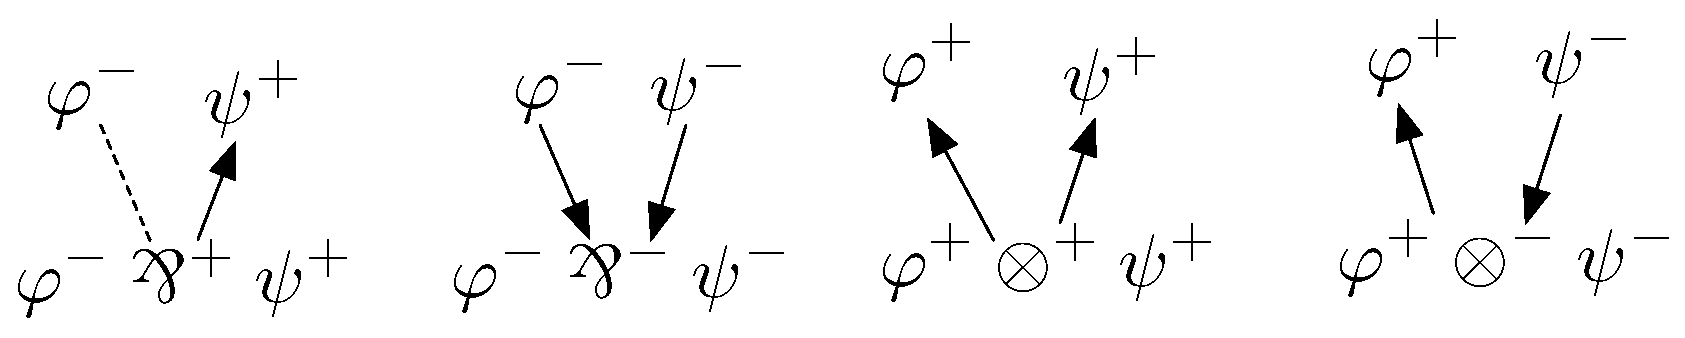
\includegraphics[scale=0.4]{rules-original.eps}
 \end{center}
For brevity, we sometimes write only the top connectives of labelling
formulae.
In that case, these branching nodes are denoted like this.
 \begin{center} %rules
  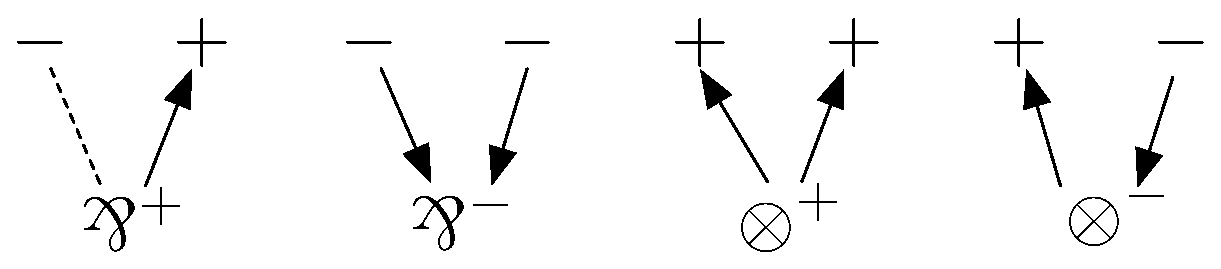
\includegraphics[scale=0.4]{rules.eps}
 \end{center}
We call arrows with upward (resp. downward) signs
\textit{up-edges}\index{up-edge}
(resp. \textit{down-edges}\index{down-edge}).
The dashed child of a $\parr^+$ node~$p$ is the node which the dashed
line from $p$ reaches.
The branching nodes labelled by $\parr^+, \parr^-, \otimes^+$ and
$\otimes^-$ are called \textit{operator nodes}.

When we add axiom edges, $\zero$-branches (shown below)
and some other operator nodes (shown above)
we obtain an
essential net of $\phi$.
Due to the arbitrarity of choosing axioms and $0^-$-branches,
there are more than one essential nets for a formula%
\footnote{\citet{murawski2003} restricts the class of formulae to linearly balanced
formulae so that the essential net is uniquely determined.}.
 \begin{center}
  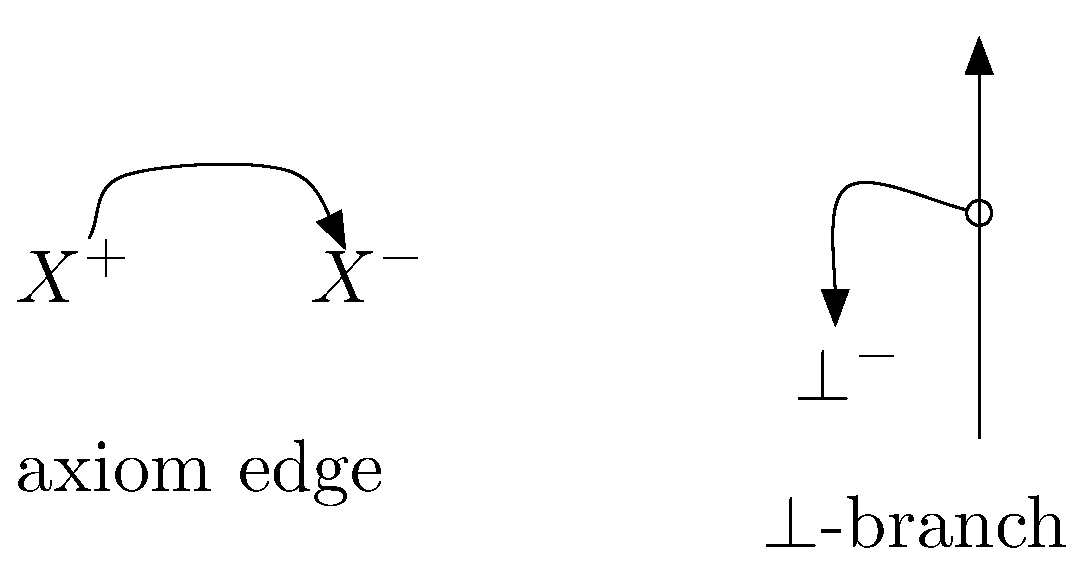
\includegraphics[scale=0.4]{axiom-cut.eps}
 \end{center}

 \begin{example}[An essential net of the Amida axiom] \label{essential-amida}
  Here is one of the essential nets of
  the Amida axiom $(X^-\parr^+Y^+)\otimes^+(Y^-\parr^+ Y^+)$.
  \fix{add}
 \end{example}

  \begin{definition}[Correct essential nets]
\begin{enumerate}
 \item Any leaf labelled with $X^+$ (resp. $Y^-$) is connected to a
       unique leaf labelled with $X^-$ (resp. $Y^+$).
       Any leaf labelled with $0^-$ is connected to an up-edge
       ($\one^+$ does not have to be connected to anything.)
 \item The directed graph formed by up-edge, down-edge, axiom edges and
       0-branches is acyclic.
 \item \label{conditionL}
       for every $\parr^+$-node~$p$, every path from the root that reaches
       $p$'s dashed child also passes through $p$.
\end{enumerate}
  \end{definition}
The essential net in Example~\ref{essential-amida} is not correct for
condition~\ref{conditionL}.  Actually, Amida axiom does not have
any correct essential net.

 \begin{theorem}[\citet{lamarche2008,murawski2003}]
  An IMLL formula~$\phi$ is provable iff there exists a correct essential net
  of $\phi$.
 \end{theorem}
 \begin{proof}
  \citet{lamarche2008} uses a common technique of decomposing an
  essential net from the bottom.
  \citet{murawski2003} chose to reduce the problem to sequents of special forms
  called regular.
 \end{proof}

 Actually, Lamarche also considers the cut rule\footnote{As well as
 additive operators and exponentials.} in essential nets, thus
 we can use the following generalized axioms (as macros) and cuts:
 \begin{center}
  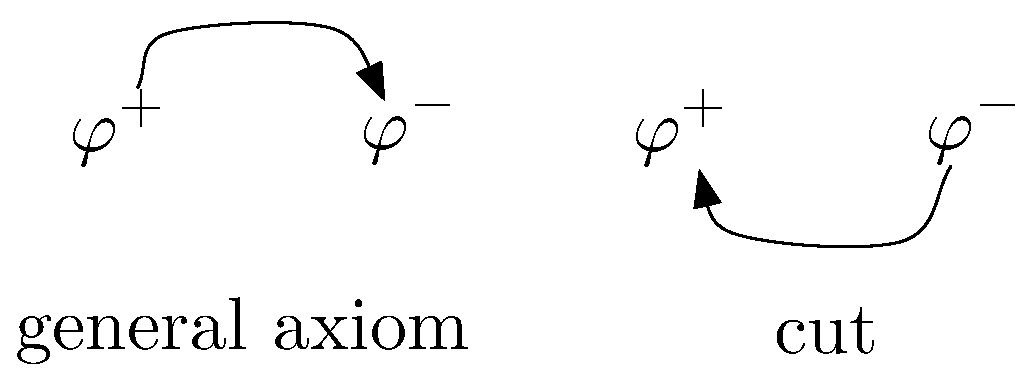
\includegraphics[scale=0.4]{general-axiom-cut.eps}\enspace.
 \end{center}

\subsection{Amida Nets}

 \begin{definition}[Amida nets]
For a hypersequent~$\hyper$,
\textit{Amida nets}\index{Amida nets} of $\hyper$ are inductively
  defined as
\begin{itemize}
 \item an essential net of $\hyper$ is an Amida net of $\hyper$
 \item for an Amida net of $\hyper$ with two different $+$~edges,
	\begin{center}
	 % twoedges
	 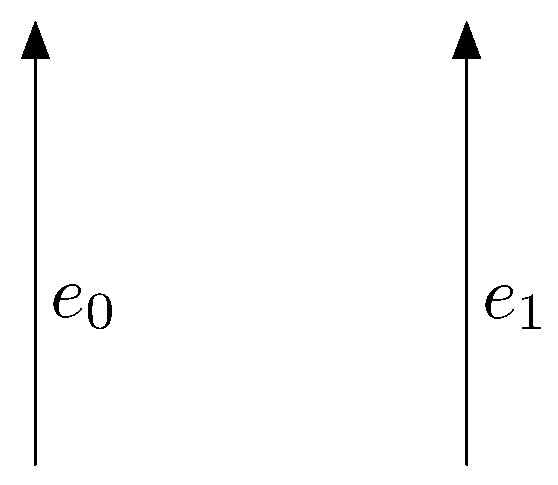
\includegraphics[scale=0.4]{twoedges.eps}
	\end{center}
       replacing these with
	\begin{center}
	 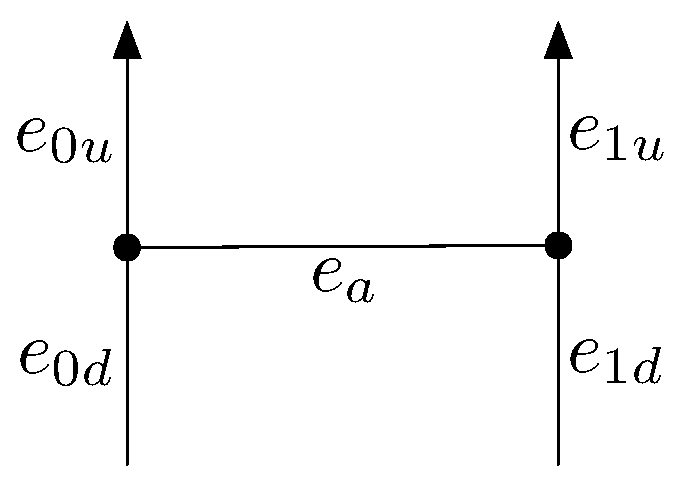
\includegraphics[scale=0.4]{twoedges_amida.eps}
	\end{center}
       yields an Amida net of $\hyper$,
       where the above component has two paths $e_{0d} e_a e_{1u}$
       and $e_{1d} e_a e_{0u}$.
 \item for an Amida net of $\hyper$ with a $+$~edge,
	\begin{center}
	 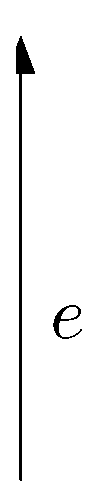
\includegraphics[scale=0.4]{oneedge.eps}
	\end{center}
       replacing these with
	\begin{center}
	 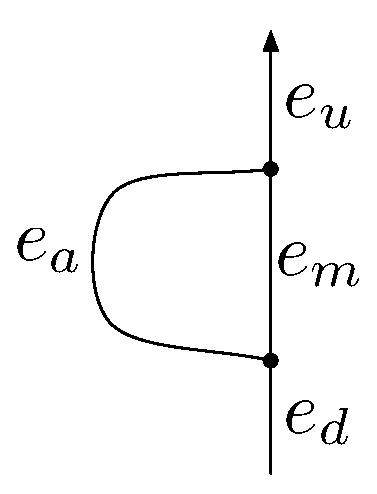
\includegraphics[scale=0.4]{oneedge_amida.eps}
	\end{center}
       yields an Amida net of $\hyper$,
       where the above component has
       one finite path $e_de_ae_u$
       and one infinite path $\cdots e_m e_a e_m e_a \cdots$.
\end{itemize}
 \end{definition}

  \begin{definition}[Correct Amida nets]
   \fix{define correct Amida nets}
  \end{definition}

 The Amida edge is not merely a crossing of vertical edges.
 See the difference between
 \begin{center}
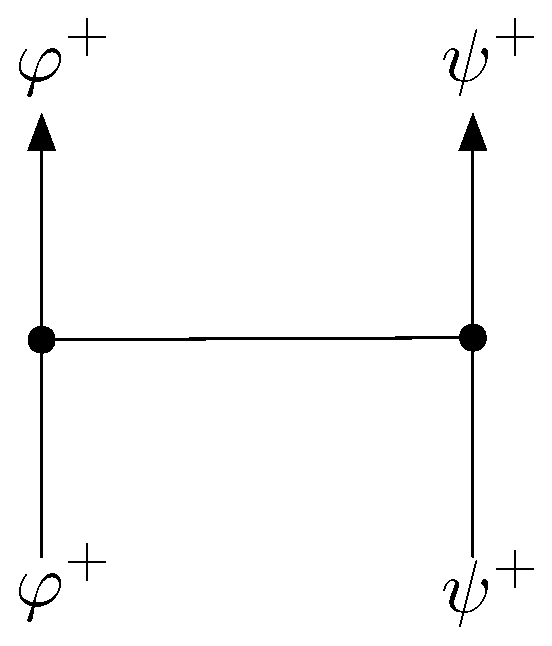
\includegraphics[scale=0.4]{twoedges_amida_without_label.eps}
 \end{center}
and
 \begin{center}

\includegraphics[scale=0.4]{crossing.eps}
 \end{center}
The difference is the labels at the bottom.
Although Amida edges cross the paths,
they do not transmit labels.
This difference causes Amida nets to validate Amida axiom.
 \begin{example}
  The Amida net for the Amida axiom $(X\limp Y)\otimes(Y\limp X)$.
   \begin{center}
    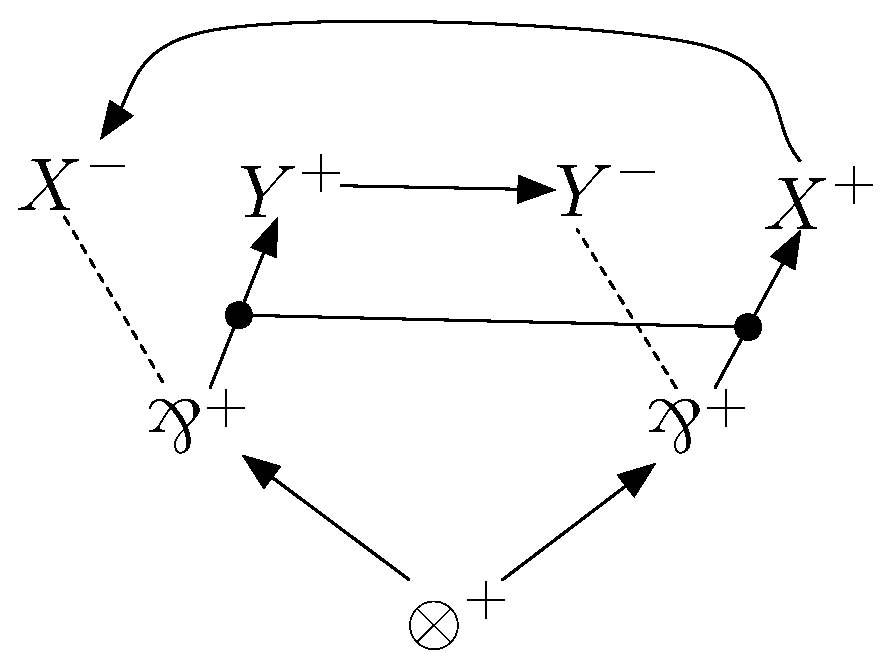
\includegraphics[scale=0.4]{amida-axiom.eps}
   \end{center}
  In terms of the set of paths, the above Amida net is equivalent to the
  following essential net for $(X\limp X)\otimes (Y\limp Y)$.
   \begin{center}
    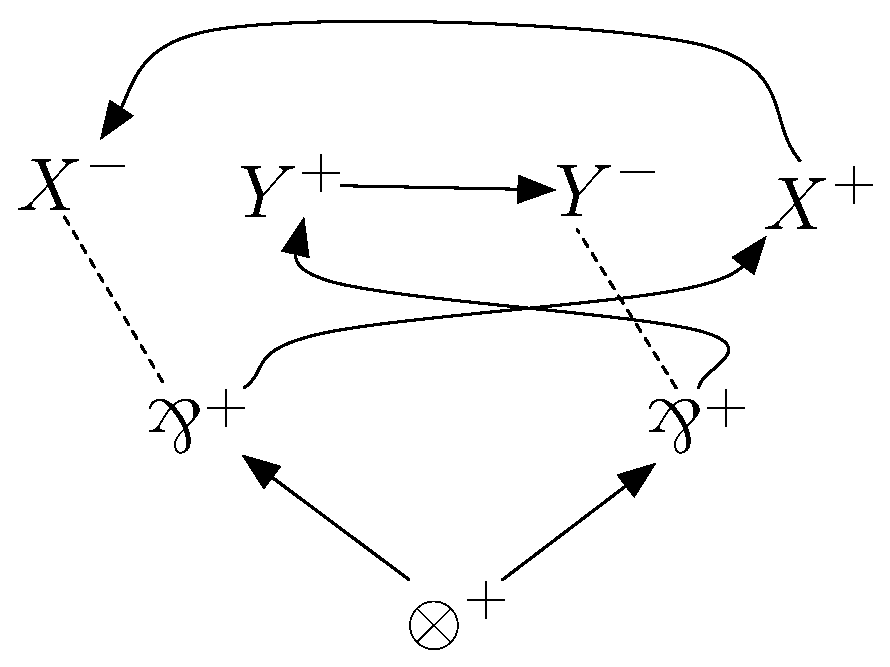
\includegraphics[scale=0.4]{amida-axiom-cross.eps}
   \end{center}
 \end{example}

\subsection{Soundness and Completeness of Amida nets}

\fix{define some words below}

 \begin{proposition}[Completeness]
  If a hypersequent $\hyper$ is derivable,
  there is a correct Amida net for $\hyper$.
 \end{proposition}
 \begin{proposition}
  Inductively on the derivation of $\hyper$,
  we can translate a sequent calculus proof into a correct Amida net.
 \end{proposition}

 Soundness is more complicated.
Inverse, from a correct Amida net, first we move the Amida edges upwards
until they are just below axiom edges.

The translation moves are as follows.
 \begin{center}
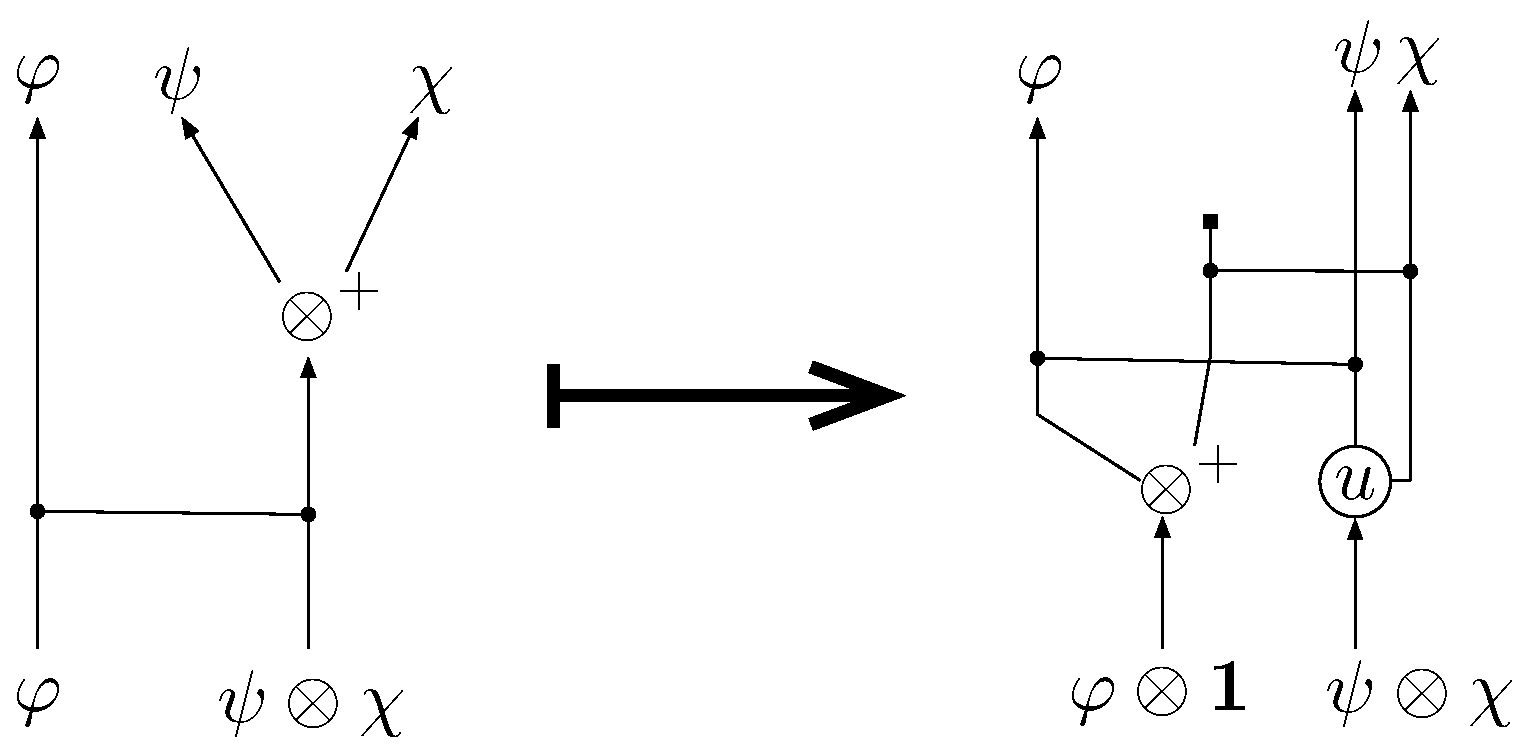
\includegraphics[scale=0.4]{tensor-move.eps}
\\
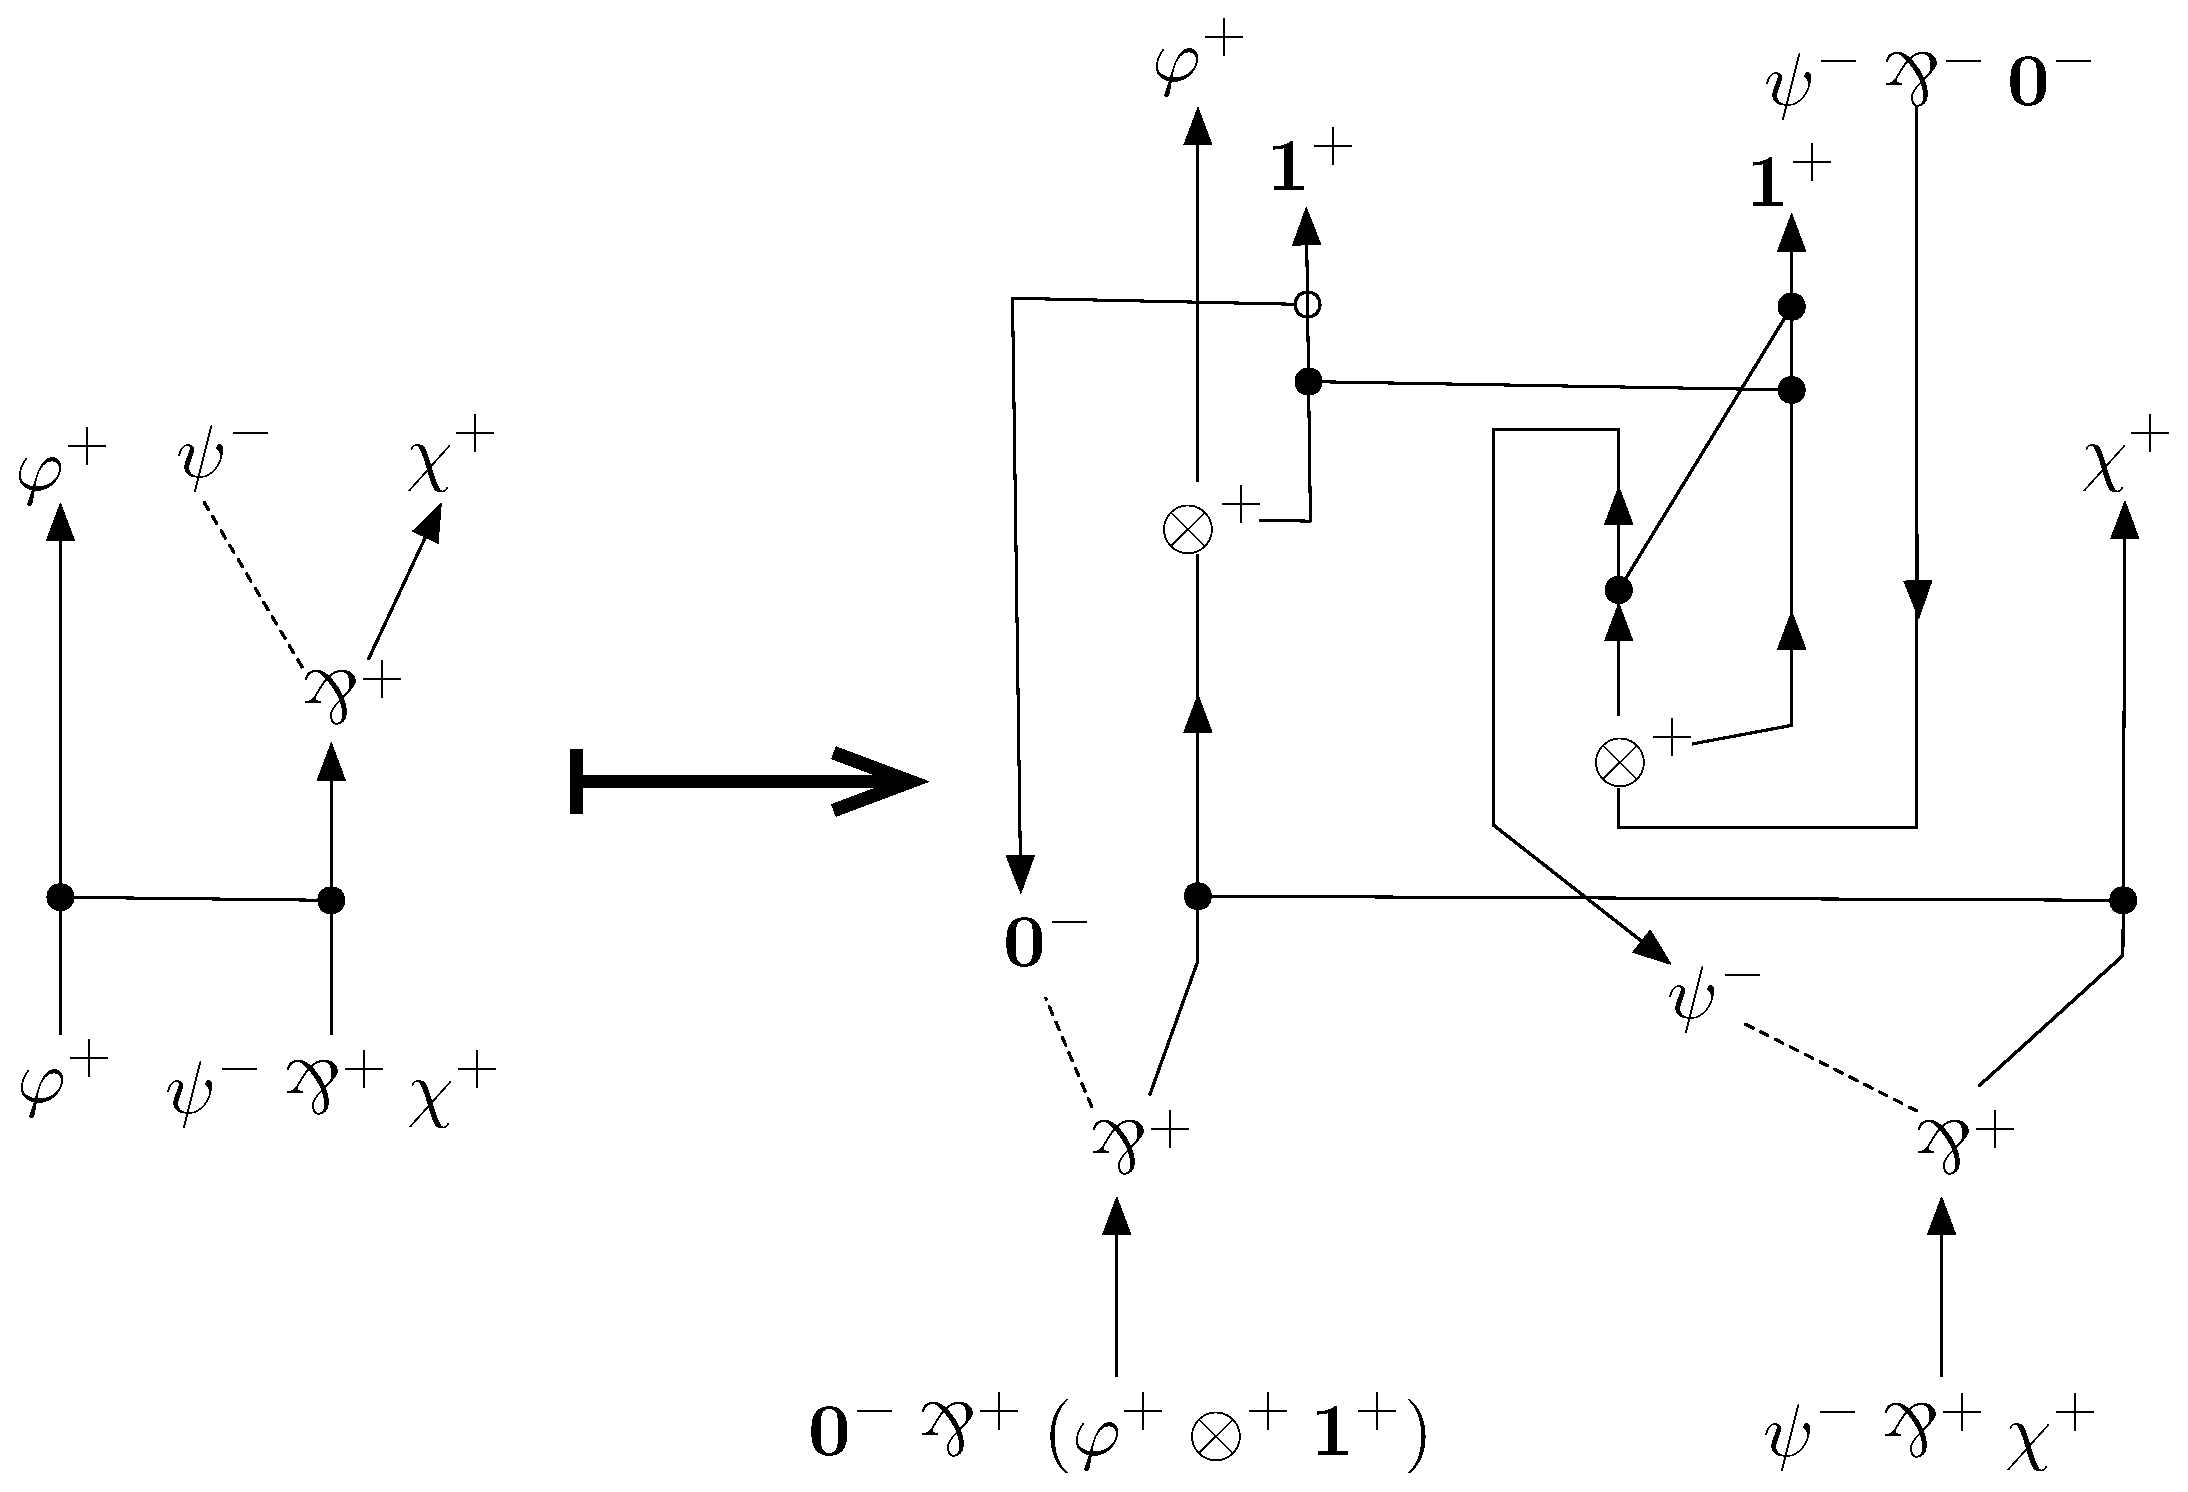
\includegraphics[scale=0.35]{parr-move.eps}
 \end{center}
These translations have two properties.
\begin{enumerate}
 \item When the original (substituted to a larger picture)
       is a correct Amida net, the translation (substituted to the same
       larger picture) is also a correct Amida net.
 \item The endpoints of the translation corresponds to the endpoints of
       the original, and the corresponding endpoints have the same label
       (up to logical equivalence in IMLL).  In case of $\otimes$
       translation, $\phi$ and
       $\phi\otimes \one$ are logically equivalent because $\one$ is the
       unit of $\otimes$.
       In case of $\parr$ translation, $\phi$ and $0\parr \phi$ are
       logically equivalent because $0$ is the unit of $\parr$.
\end{enumerate}
For checking the first condition, it is enough to follow the paths
(crossing all Amida edges).
For the second condition, it is enough to follow the vertical edges
except the Amida edges.

The $\otimes$ move introduces Amida edges only above the branching rules.
Although the $\parr$ move introduces an Amida edge below a
branching rule, that branching rule is of $\otimes$ nature.
Also, the $\parr$ move introduces an Amida edge below $\psi$-axiom link,
which is actually a macro.  So we have to continue applying the
translation moves in the macro.  However, Since $\psi$ is a strictly
smaller subformula of $\psi\parr\chi$, this does not cause infinite
recursion.

Then, by these translation moves,
the whole Amida net is decomposed vertically into three layers.
At the top, there is a layer with only Axiom edges.
In the middle, there is a layer with only vertical edges and Amida
edges.
At the bottom, there is a layer which contains only ordinary
essential net nodes.

Since the middle layer is an Amida lottery, it defines a permutation.
That permutation can be expressed as a product of transpositions, so
that
the original Amida lottery is equivalent to a loop-less Amida lottery.
A loop-less Amida lottery is an encoding of a hypersequent derivation
that consists of only Sync rules.

After we encode the top and the middle layer, encoding the bottom layer
is the same as \fix{Lamarche's theorem which}


We expect that it is possible to add Amida edges to
the full intuitionistic logic following
\citet{groote1999}
\fix{cite de groote / cite Lamarche}


\section{Related Work}

One promising approach is using session types~\citep{honda-session}.
Session types aims at typing channels and processes in $\pi$-calculus so
that the process execution is deterministic and not ending in deadlock.
In general session type systems are not based on well-known logic.


\fix{mention join calculus here or in related work}


\subsection{Pfenning}

\citet{pfenning2010} provide a type system for a fragment of $\pi$-calculus.
Their type system imposes too strong a discipline
than necessary to provide deadlock freedom.
The escrowing process $P$ below is not typable in their type
system:
\[
 P = \sendterm x y{\recvterm x a {\recvterm y b {\sendterm x b
 {\sendterm y a 0}}}}\enspace.
\]
The process first emits a channel~$y$ through channel~$x$ and then
exchanges inputs from $x$ and $y$ into outputs to $y$ and $x$.
Following the informal description of types in \citep{pfenning2010},
the process~$P$ should be typable as
\[
 \vdash P::x:(A\limp B)\otimes(B\limp A)\enspace.
\]
However, such typing is not possible because $(A\limp B)\otimes (B\limp
A)$ is not a theorem of \fix{name} (DILL), the logic their type system
is based on.
In our type system, the following sequent is derivable
\begin{align*}
&
\tj{x}{\sendtype{\sendtype{B}{\recvtype{A}\terminate}}{\recvtype B
{\sendtype A \terminate}}}
\tr\\
&\tj{
\nu(\tj{y}{\sendtype B{\recvtype A \terminate}}).
{\sendterm x{y_L}{\recvterm x a {\recvterm {y_R} b {\sendterm x b {\sendterm
{y_R} a {\ign{x,y}0}}}}}}
}{\one}
\end{align*}
The resulting sequent indicates that the process is typable with one
open channel~$x$ that emits
a channel to/from which one can send~$B$ and receive~$A$, receives a
value of $B$ and
sends a value of $A$.
This example shows that our type system is strictly more flexible than
the type system in \citet{pfenning2010}.
Moreover, we still ensure deadlock freedom in the sense that all typed
processes reduce to the canonical form~(\thref{convergence}).

The most complicated example in \citet{pfenning2010} is the following
one, which can be typed and evaluated in our framework as well.

 \begin{example}[Drink server example from \citet{pfenning2010}]
  \begin{align*}
   ServerProto &= (N\limp I \limp (N\otimes \one))\with (N\limp( I
  \otimes \one)) \\
   &= (\sendtype N {\sendtype { I} {\recvtype N \terminate}}) \with
   (\sendtype N {\recvtype { I} \one})
  \end{align*}
  $N$ stands for the type of strings and $I$ stands for the type of
  integers, but following \citet{pfenning2010}, we identify both $N$ and
  $I$ with $\one$.
  Here is the prototype of the server, that serves one client and
  terminates.\\
  \[
   Serv = \lpair{\recvterm s {pn} {\recvterm s {cn} {\sendterm s {rc}
  {\ign {pn, cn, s} 0}}}
  ,\quad
  \recvterm s {pn} {\sendterm s {pr} {\ign{s,pn} 0}}
  }
  \]
  We can derive a sequent $\tj{s}{\overline{SP}}\tr\tj{Serv}\one$.
  \fix{how}

  Using this, we can also implement a server that can replicate itself
  and serve many clients.  Below, $SP$ abbreviates $ServerProto$.
  \begin{center}
   \AxiomC{$\tj{s}{\overline{SP}}\tr\tj {Serv}{\one}$}
   \AxiomC{}
   \UnaryInfC{$\tj{x}{SP}\tr\tj{x}{SP}$}
   \UnaryInfC{$\tj{z}\one,\tj{x}{SP}\tr\tj{\ign z x}{SP}$}
   \BinaryInfC{$\tj{s}{\overline{SP}},\tj{x}{SP}\tr\tj{\ign{Serv}x}{SP}$}
   \UnaryInfC{$\tr\tj{\nu(\tj{s}{SP}).\ign{Serv[s_R/s]}{s_L}}{SP}$}
   \UnaryInfC{$\tr\bang\tj{\nu(\tj{s}{SP}).\ign{Serv[s_R/s]}{s_L}}{\bang
   SP}$}
   \DisplayProof
  \end{center}


  Here is one client:
  \begin{center}
   \AxiomC{}
   \UnaryInfC{$\tr\tj{0}\one$}
   \UnaryInfC{$\tj{s}{\terminate}\tr\tj{\ign s 0}\one$}
   \UnaryInfC{$\tj{s}{\terminate},
   \tj{pr}{I}\tr\tj{\ign{pr,s} 0}\one$}
   \UnaryInfC{
   $ \tj{s}{\recvtype {I} {\terminate}} \tr\tj{
   \recvterm s {pr} {\ign{pr,s} 0}
   }{\one}$
   }
   \AxiomC{}
   \UnaryInfC{$ \tr\tj{tea}{N} $}
   \BinaryInfC{
   $ \tj{s}{\sendtype N {\recvtype {I} \terminate}} \tr\tj{
   \sendterm s {tea}
   {\recvterm s {pr} {\ign{pr,s} 0}}
   }{\one}$
   }
   \UnaryInfC{
   $ \tj{s}{ServerProto} \tr\tj{
   \letin s {\lpair{\_, s}} {
   \sendterm s {tea}
   {\recvterm s {pr} {\ign{pr,s} 0}}}
   }{\one}$
   }
   \DisplayProof
  \end{center}
  We abbreviate the process as $QClnt_s$.
  In words, the client first chooses the server's second protocol, which
  is price quoting, and asks the price of the tea, receives the price
  and terminates.

  Here is another client.
  \begin{center}
   \AxiomC{}
   \UnaryInfC{$ \tr\tj{0}\one $}
   \UnaryInfC{$ \tj{s}{\terminate}\tr\tj{\ign s 0}\one$}
   \UnaryInfC{$ \tj{s}{\terminate},\tj{rc}{N}\tr\tj{
   {\ign {rc,s} 0}}\one$}
   \UnaryInfC{$ \tj{s}{\recvtype{N}\terminate}\tr
   \tj
   {\recvterm{s}{rc}{\ign {rc,s} 0}}
   {\one}$}
   \AxiomC{}
   \UnaryInfC{$\tr\tj{pin}{I}$}
   \BinaryInfC{$ \tj{s}{\sendtype{I}{\recvtype{N}\terminate}}\tr
   \tj
   {\sendterm{s}{pin}{\recvterm{s}{rc}{\ign {rc,s} 0}}}
   {\one}$}
   \UnaryInfC{$ \tj{s}{\sendtype{N}{\sendtype{I}{\recvtype{N}\terminate}}}\tr
   \tj
   {\sendterm{s}{cof}{\sendterm{s}{pin}{\recvterm{s}{rc}{\ign {rc,s} 0}}}}
   {\one}$}
   \UnaryInfC{$ \tj{s}{ServerProto}\tr
   \tj
   {\letin s {\lpair{s,\_}}
   {\sendterm{s}{cof}{\sendterm{s}{pin}{\recvterm{s}{rc}{\ign {rc,s} 0}}}}}
   {\one}$}
   \DisplayProof
  \end{center}
  We abbreviate the process as $BClnt_s$.

  We can combine the server with two clients.
   \begin{center}
    \AxiomC{$\tj{s}{SP}\tr\tj{QClint_s}{\one}$}
    \AxiomC{$\tj{s'}{SP}\tr\tj{BClint_{s'}}{\one}$}
    \BinaryInfC{$\tj{s}{SP},\tj{s'}{SP}\tr
    \tj{{QClint_s}\otimes{BClint_{s'}}}{\one\otimes\one}$}
    \UnaryInfC{$\tj{s}{!SP},\tj{s'}{!SP}\tr
    \tj{\letin{s}{!s}{\letin{s'}{!s'}
    {{QClint_s}\otimes{BClint_{s'}}}}}{\one\otimes\one}$}
    \UnaryInfC{$\tj{s}{!SP}\tr
    \tj{\letin{s}{s@s'}{
    \letin{s}{!s}{\letin{s'}{!s'}
    {{QClint_s}\otimes{BClint_{s'}}}}}}{\one\otimes\one}$}
    \UnaryInfC{$\tr
    \tj{\letin{!Serv}{s@s'}{
    \letin{s}{!s}{\letin{s'}{!s'}
    {{QClint_s}\otimes{BClint_{s'}}}}}}{\one\otimes\one}$}
    \DisplayProof
   \end{center}

  Here is an evaluation of the combined system of the server and the two
  clients.
 \end{example}

\subsection{Wadler}

\citet{wadler2012propositions} gave a type system for a process
calculus based on classical linear logic.
Although the setting is classical, the idea is more or less the same as
\citet{pfenning2010}.
Wadler's type system cannot type the escrowing process above.
Worse, \citet{wadler2012propositions} does not recognize this
\[
 \sendterm x y{\recvterm x a {\recvterm y b {\sendterm x b {\sendterm y
 a 0}}}}
\]
as a process at all.
His grammar requires the output construction to be used in the form
\[
 \sendterm x y {(P\mid Q)}
\]
where $x$ is bound in $Q$ but not in $P$ and $y$ is bound in $P$ but not
in $Q$.
Of course, there is a way to escape the above restriction by making $P$
and $Q$ communicate, but that option is prohibited by the typing rules.

Wadler uses classical linear logic rather than intuitionistic linear
logic.
He justifies the choice for ``greater simplicity and symmetry.''
Adding Amida axiom to the classical linear logic is a future direction.
One looming difficulty is as follows.
In classical multiplicative linear logic,
adding Amida edges to proof nets seems harder than the intuitionistic case
because classical MLL proof nets have no direction on edges.
After a path crosses an Amida edge, the author has no idea which
direction the path should continue.

In other respects,
Wadler's type system is similar to ours;
our abbreviations are largely taken from Wadler's translations.

\subsection{Beffara}

\subsection{Giunti and Vasconcelos}

\citet{giunti2010} gives a type system for the pi calculus, which is
extremely similar to our type system.
They say ``the goale of this work is to equip types with a contsructor
able to denote the two ends of a same
channel.''~\citep[Introduction]{giunti2010}
One of their typing rules
 \begin{center}
  \AxiomC{$\G,x\colon(S,\overline S)\tr P$}
  \UnaryInfC{$\G\tr(\nu x)P$}
  \DisplayProof
 \end{center}
 is similar to a rule in \thref{typing_connection}
 \begin{center}
  \AxiomC   {$\hypert\hmid
  \G,\tj{x}{\phi^\ell},\tj{y}{\overline{\phi^\ell}}\tr\tj t \psi$}
  \UnaryInfC{$\hypert\hmid
  \G\tr\tj{\nu\tj{x}{\phi^\ell}.t[x_L/x][x_R/y]}{\psi}$}
  \DisplayProof\enspace.
 \end{center}
 Usually, the Curry--Howard correspondence is followed from logical world
 to the programming world: for an alraedy known logic, a new lambda
 calculus is invented (e.g.~\fix{lambda mu kakutani kimura pfenning alex
 sympson so on}).  However, in our case, it seems that we have just
 found a logic called Amida logic that corresponds to an already known
 typing descipline invented by \citet{giunti2010}.
 It will be worthwhile to compare their system with our type system.

 \subsection{Double Binder}
 Our $\nu x$ notation binds two variables $x_L$ and $x_R$.
 This is similar to the double binder $\nu x_L x_R$ appearing in
 \citet{gay2010}.

 \subsection{Logic Programming}

 There are at least two ways to interpret logics computationally.
 One is proof reduction, which is represented by $\lambda$-calculi.
 The other is proof searching.  What is the meaning of Amida axiom in
 the proof searching approach?

 Let us cite an example from \citet[A.2]{kobayashi-yonezawa}:
 \begin{quote}
  Consumption of a message $m$ by a process $m\limp B$ is represented by
  the following deduction:
  \[
   (m\otimes(m\limp B)\otimes C)\limp (B\otimes C)
  \]
  where $C$ can be considered as other processes and messages, or an environment.
 \end{quote}
 In existence of Amida axiom,
 the inverse
 \[
  (B\otimes C)\limp (m\otimes (m\limp B))\otimes C
 \]
 is derivable.
 This suggests that the Amida axiom states that some
 computation is reversible.  We are not sure whether this is very
 useful within the realm of reversible computation~\citep{revcon}.

\section{Discussion}

\subsection{Categorical Considerations}
One might want to ask whether we can model the logic with
a symmetric monoidal closed category~\citep{blute2004category}
  with identified isomorphisms
$\sigma_{ABCD}\colon (A\limp B)\otimes (C\limp D)\rightarrow (A\limp D) \otimes
 (C\limp B)$, with naturality conditions.
 Before considering equality among morphisms,
 we know there is a non-trivial example.
  \begin{example}[A symmetric monoidal closed category with swaps]
   The preorder formed by objects as integers and morphisms as the usual
   order among integers~$\le$
   forms a symmetric monoidal closed category with swaps
   when we interpret $\otimes$ as addition,
   $m \limp n$ as $n-m$.
  \end{example}
  On the other hand,
  if we take another formulation requiring natural isomorphisms
  $\mathcal C(C,A)\times\mathcal C(D,B) \cong \mathcal C(D,A)\times
  \mathcal C{(C,B)}$,
  only singletons can be preorder models because $\tuple{id_A,id_B}$ is
  mapped to $\tuple{f,g}$ where $f\colon A\rightarrow B$ and $g\colon
  B\rightarrow A$ for any two objects $A$ and $B$.

A straightforward reading of evaluation rules gives somewhat complicated
equality conditions for morphisms.
The condition says the following diagram commutes:
\[
   \begin{CD}
    (A\limp B)\otimes (C\limp D) @>{d_{ABCD}}>> (A\otimes C)\limp(B\otimes D)\\
    @VV{\sigma_{ABCD}}V @VV{id\limp s_{B,D}}V\\
    (A\limp D)\otimes (C\limp B) @>{d_{ADCB}}>> (A\otimes C)\limp (D\otimes B)
   \end{CD}
\]
where $d_{ABCD}$ is induced by adjunction between $\otimes$ and $\limp$
 from a morphism
 $((A\limp B)\otimes (C\limp D))\otimes (A\otimes C)\rightarrow
 (B\otimes D)$, which is provided by symmetric monoidal closed
 properties.

 \subsection{Logical Considerations}

 When we add
 the intuitionistic version of Amida axiom
 $(\phi\imp\psi)\land(\psi\imp\phi)$ to the intuitionistic propositional
 logic,
 the logic becomes inconsistent.
 Actually,
 if we have weakening, we can derive $(\phi\land \psi)\imp \phi$ so that
 we can throw away half of the Amida axiom
 $(\phi\imp\psi)\land(\psi\imp\phi)$ to obtain $\phi\imp\psi$ for any
 $\phi$ and $\psi$.  Thus we can conclude that Amida axiom is
 inconsistent with weakening.

 On the other hand, from the operational perspective, we expect Amida
 axiom to be consistent with contraction.
 We reckon that relevant Amida logic can be studied, but
 it is a mystery whether such a logic is philosophically relevant.

\subsection{Multiparty, recursions, \ldots}
We expect it straightforward to add recursions in our type system.
As a guidance we can take $\mu$MALL of \citet{mumall}.

Our operational semantics is different from the standard session
calculus.  Since our operational semantics seems more liberal,
if we limit it, we do not lose type safety.  However, if we do not
choose a suitable class of reductions, the reduction can be
nondeterministic.
The reconcilation of lienarity and pi-calculus style operational
semantics has already been considered by
\citet{kobayashi-pierce-turner} so we expect their work to be a
guidance toward finding a more traditional operational semantics.

It is tempting to add modalities showing agents to types so that the
modalities show agents and then study the relationship with the
multiparty session types~\citep{sync-multi-session, async-multi-session}.
For that, intuitionistic epistemic logic~\citet{hirailpar,hiraimaster}
will be useful.

\section{Conclusion}

We found Amida logic, which can be characterized by Amida axiom
$(\phi\limp\psi)\otimes(\psi\limp\phi)$ on top of intuitionistic
linear logic.
The logic has an application for encoding process calculi and session type
system.
As a technique, we first used conjunctive hypersequents,
where components in a hypersequent are interpreted conjunctively rather
than disjunctively.